%\setcounter{chapter}{3}
\chapter{Imaging}\index{Imaging}
\label{chapter:imaging}


\section{Introduction}

Light sources, like the sun or artificial lights, flood our world with light rays.   These reflect off surfaces, generating a field of light rays heading in
all directions through space.  As the light rays reflect from the surfaces,
they generally change in some attributes, such as their brightness or their color.  It is those changes, after reflection from a surface, that let us interpret what we see. In this chapter, we describe how light interacts with surfaces and how those interactions are recorded with a camera.


\section{Light Interacting with Surfaces}
\label{sec:light_interacting_with_surfaces}
Visible light is electromagnetic radiation, exhibiting wave effects like diffraction.  For many imaging models, however, it is helpful to introduce the abstraction of a {\bf light ray}\index{Light ray}, describing the light radiation heading in a particular direction from a particular location in space (\fig{\ref{fig:lightSpray}}).  A light ray is specified by its position, direction, and intensity as a function of wavelength and polarization.  In this treatment, we ignore diffraction effects.

%\begin{comment}
\begin{figure}
\centerline{
\includegraphics[width=0.7\linewidth]{figures/imaging/brdf.eps}}
\caption{A light ray from the sun strikes a surface and generates outgoing rays of intensity and color depending on the angles of the incoming and outgoing rays relative to the surface orientation.}
\label{fig:lightSpray}
\end{figure}
%\end{comment}

Let an incident light ray be from direction $\mathbf{p}$ and
of power, $\imgin(\lambda)$, as a function of spectral wavelength $\lambda$ (\fig{\ref{fig:lightSpray}}).  The
power of the outgoing light, reflected in the direction, $\mathbf{q}$, is determined by what is called the {\bf bidirectional
reflection distribution function}\index{BRDF} (BRDF), $F$, of the surface. If the
surface normal is $\mathbf{n}$, then  outgoing power is some function, $F$, of the surface normal, the incoming and outgoing ray directions, the wavelength, and the incoming light power:
\begin{equation}
\imgout = F \left( \imgin, \mathbf{n}, \lambda, \mathbf{p}, \mathbf{q} \right)
\label{eq:Lambert}
\end{equation}

\subsection{Lambertian Surfaces}

In general, BRDFs can be quite complicated (see \cite{Matusik2002}), describing both diffuse and specular components of reflection.  Even surfaces with completely diffuse reflections can give complicated reflectance distributions \cite{Oren1994}.  
A useful approximation describing diffuse reflection is the {\bf Lambertian model}\index{BRDF!Lambertian}, with a particularly simple BRDF, which we denote as $F_L$.  The outgoing ray intensity, $\imgout$, is a function only of the surface orientation relative to the incoming and outgoing ray directions, the wavelength, a scalar surface reflectance, and the incoming light power:
\begin{equation}
%I_{\mbox{out}} = F_{L}(I_{\mbox{in}} (\lambda), \mathbf{n}, \mathbf{p})  = a I_{\mbox{in}}(\lambda) \cos(\mathbf{n} \cdot \mathbf{p}),
\imgout = F_{L} \left( \imgin (\lambda), \mathbf{n}, \mathbf{p} \right)  = a \imgin(\lambda) \left( \mathbf{n} \cdot \mathbf{p} \right),
\label{eq:lambert}
\end{equation}
where $a$ is the surface {\bf reflectance}, or {\bf albedo}, $\mathbf{n}$ is the
surface normal vector, and $\mathbf{p}$ points toward the source of the incident
light.  Note that the brightness of the outgoing light ray depends on
the orientation of the surface relative to the incident ray, as well
as the reflectance, $a$, of the surface.  For a Lambertian surface,
the intensity of the reflected light is a function of the direction of
the incoming light ray, but not a function of the outgoing direction
of the ray, $\mathbf{q}$.  

\marginnote{Perfectly Lambertian surfaces are not common. The synthetic material called spectralon is the most perfectly Lambertian material.}

\subsection{Specular Surfaces\index{Specular surfaces}}



A widely used model of surfaces with a specular component of reflection is the {\bf Phong reflection model}\index{BRDF!Phong model} \cite{Phong1975}.  The light reflected from a surface is assumed to have three components that result in the observed reflection:  (1) an ambient component, which is a constant term added to all reflections; (2) a diffuse component, which is the Lambertian reflection of \eqn{\ref{eq:Lambert}}; and (3) a specular reflection component. For a given ray direction, $\mathbf{q}$, from the surface, the Phong specular contribution, $\img_{\mbox{Phong spec}}$, is:
\begin{equation}
\img_{\mbox{Phong spec}} = k_s (\mathbf{r} \cdot \mathbf{q})^\alpha \imgin,
\end{equation}
where $k_s$ is a constant, $\alpha$ is a parameter governing the spread of the specular reflection, and the unit vector $\mathbf{r}$ denotes the direction of maximum specular reflection, given by
\begin{equation}
\mathbf{r} = 2(\mathbf{p} \cdot \mathbf{n}) \mathbf{n} - \mathbf{p}
\end{equation}
\Fig{\ref{fig:rendering}} shows the ambient, Lambertian, and Phong shading components of a sphere under two-source illumination, and a comparison with a real sphere under similar real illumination.


\begin{figure}[t]
\centerline{
\sublabelnp{(a) Lambertian}{\includegraphics[width=0.3\linewidth]{figures/imaging/sphereDiffuse.png}}
\sublabelnp{(b) Phong}{\includegraphics[width=0.3\linewidth]{figures/imaging/spherePhongRoughness0.3.png}}
\sublabelnp{(c) Photograph}{\includegraphics[width=0.3\linewidth]{figures/imaging/photoSphere.jpg}}}
\caption{(a and b) Two different renderings of a sphere.  (c) Note the many extra details required of a photorealistic rendering.}
\label{fig:rendering}
\end{figure}


In general, surface reflection behaves
linearly:  the reflection from the sum of two light sources is the sum of the
reflections from the individual sources. 

To associate the reflected light with surfaces in the world, we need to know which light rays came from which direction in space.  That requires that we form an image, which we discuss next.

% what happens when light hits a surface? basic radiometry
% talk about radiance, penoptic function, lightfields here?


\section{The Pinhole Camera and Image Formation}
\label{sec:pinhole_camera_formation}

Naively, we might wonder when looking at a blank wall, why we don't see an image of the scene facing that wall.  The light reflected from
the wall integrates light from every reflecting surface in the room,
so the reflected intensities are an average of light intensities from
many different directions and many
different sources, as illustrated in \fig{\ref{fig:wallpicture}}{a}.  Mathematically, integrating the equation for
Lambertian reflections (equation [\ref{eq:lambert}]) over all possible
incoming light directions $\mathbf{p}$,  we have 
for the intensity reflecting off a Lambertian surface, $\imgout$:
\begin{equation}
\imgout = \int_{\mathbf{p}}  a \imgin(\mathbf{p}) \cos(\mathbf{n} \cdot \mathbf{p}) \mbox{d} \mathbf{p}
\end{equation}
The intensity, $\imgout$, reflecting off a diffuse wall, thus tells us very little about the incoming light intensity $\imgin(\mathbf{p})$ from any given direction $\mathbf{p}$. To learn about $\imgin(\mathbf{p})$, we need to form an image.
Forming an image involves identifying
which rays came from which directions. The role of a camera is to
organize those rays, to convert the cacophony of light rays going
everywhere to a set of measurements of intensities coming from
different directions in space, and thus from different surfaces in the world.


Perhaps the simplest camera is a {\bf pinhole camera}\index{Camera!Pinhole camera}.  A pinhole camera requires a light-tight enclosure, a small hole
that lets light pass, and a projection surface where one senses or views the illumination intensity as a function of position.
\Fig{\ref{fig:wallpicture}}{b} shows the the geometry of a scene, the
pinhole, and a projection surface (wall).  For any given point on the
projection surface, the light that falls there comes from only from one direction, along the straight line joining the surface position and the pinhole.   This creates an image of what's in the world on the
projection plane.%, Figure~\ref{fig:pinhole}~(b).


\begin{figure}[t]
\centerline{
\includegraphics[width=1\linewidth]{figures/imaging/no_picture_on_a_wall_aina.eps}}
\caption{(a) Why there are no pictures appearing on the walls? (b) The pinhole camera restricts the light rays reaching the wall, producing an image to appear.}
\label{fig:wallpicture}
\end{figure}


\begin{comment}
\begin{figure}
\centerline{
\sublabel{a}{
\includegraphics[width=1\linewidth]{figures/imaging/pinhole7.pdf}}}
\centerline{\sublabel{b}{
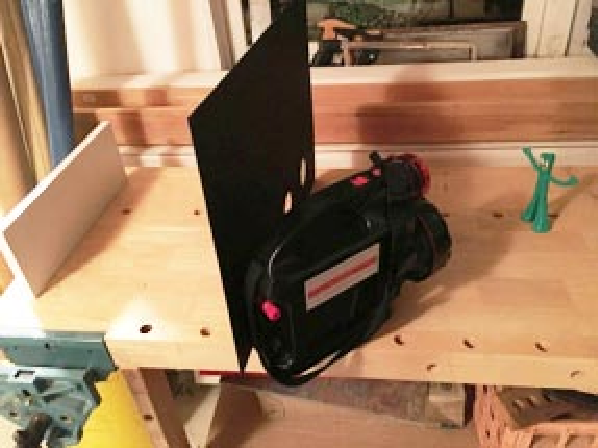
\includegraphics[width=0.5\linewidth]{figures/imaging/pinhole3.jpg}}
\sublabel{c}{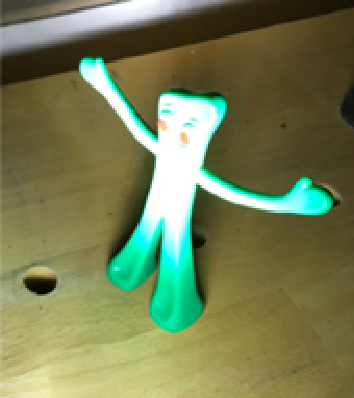
\includegraphics[width=0.3\linewidth]{figures/imaging/gumby.pdf}}}
\caption{(a) Pinhole camera geometry, showing some light rays passing
  through the pinhole aperture to the projection plane.  (b) Image on the projection plane resulting from
  lighting projecting through a pinhole from  the subject, (c). Fig.~\ref{fig:pinholeSize}~(a) shows the configuration of the object, pinhole, and projection plane.}
\label{fig:pinhole}
\end{figure}
\end{comment}

%% \centerline{
%% \sublabel{a}{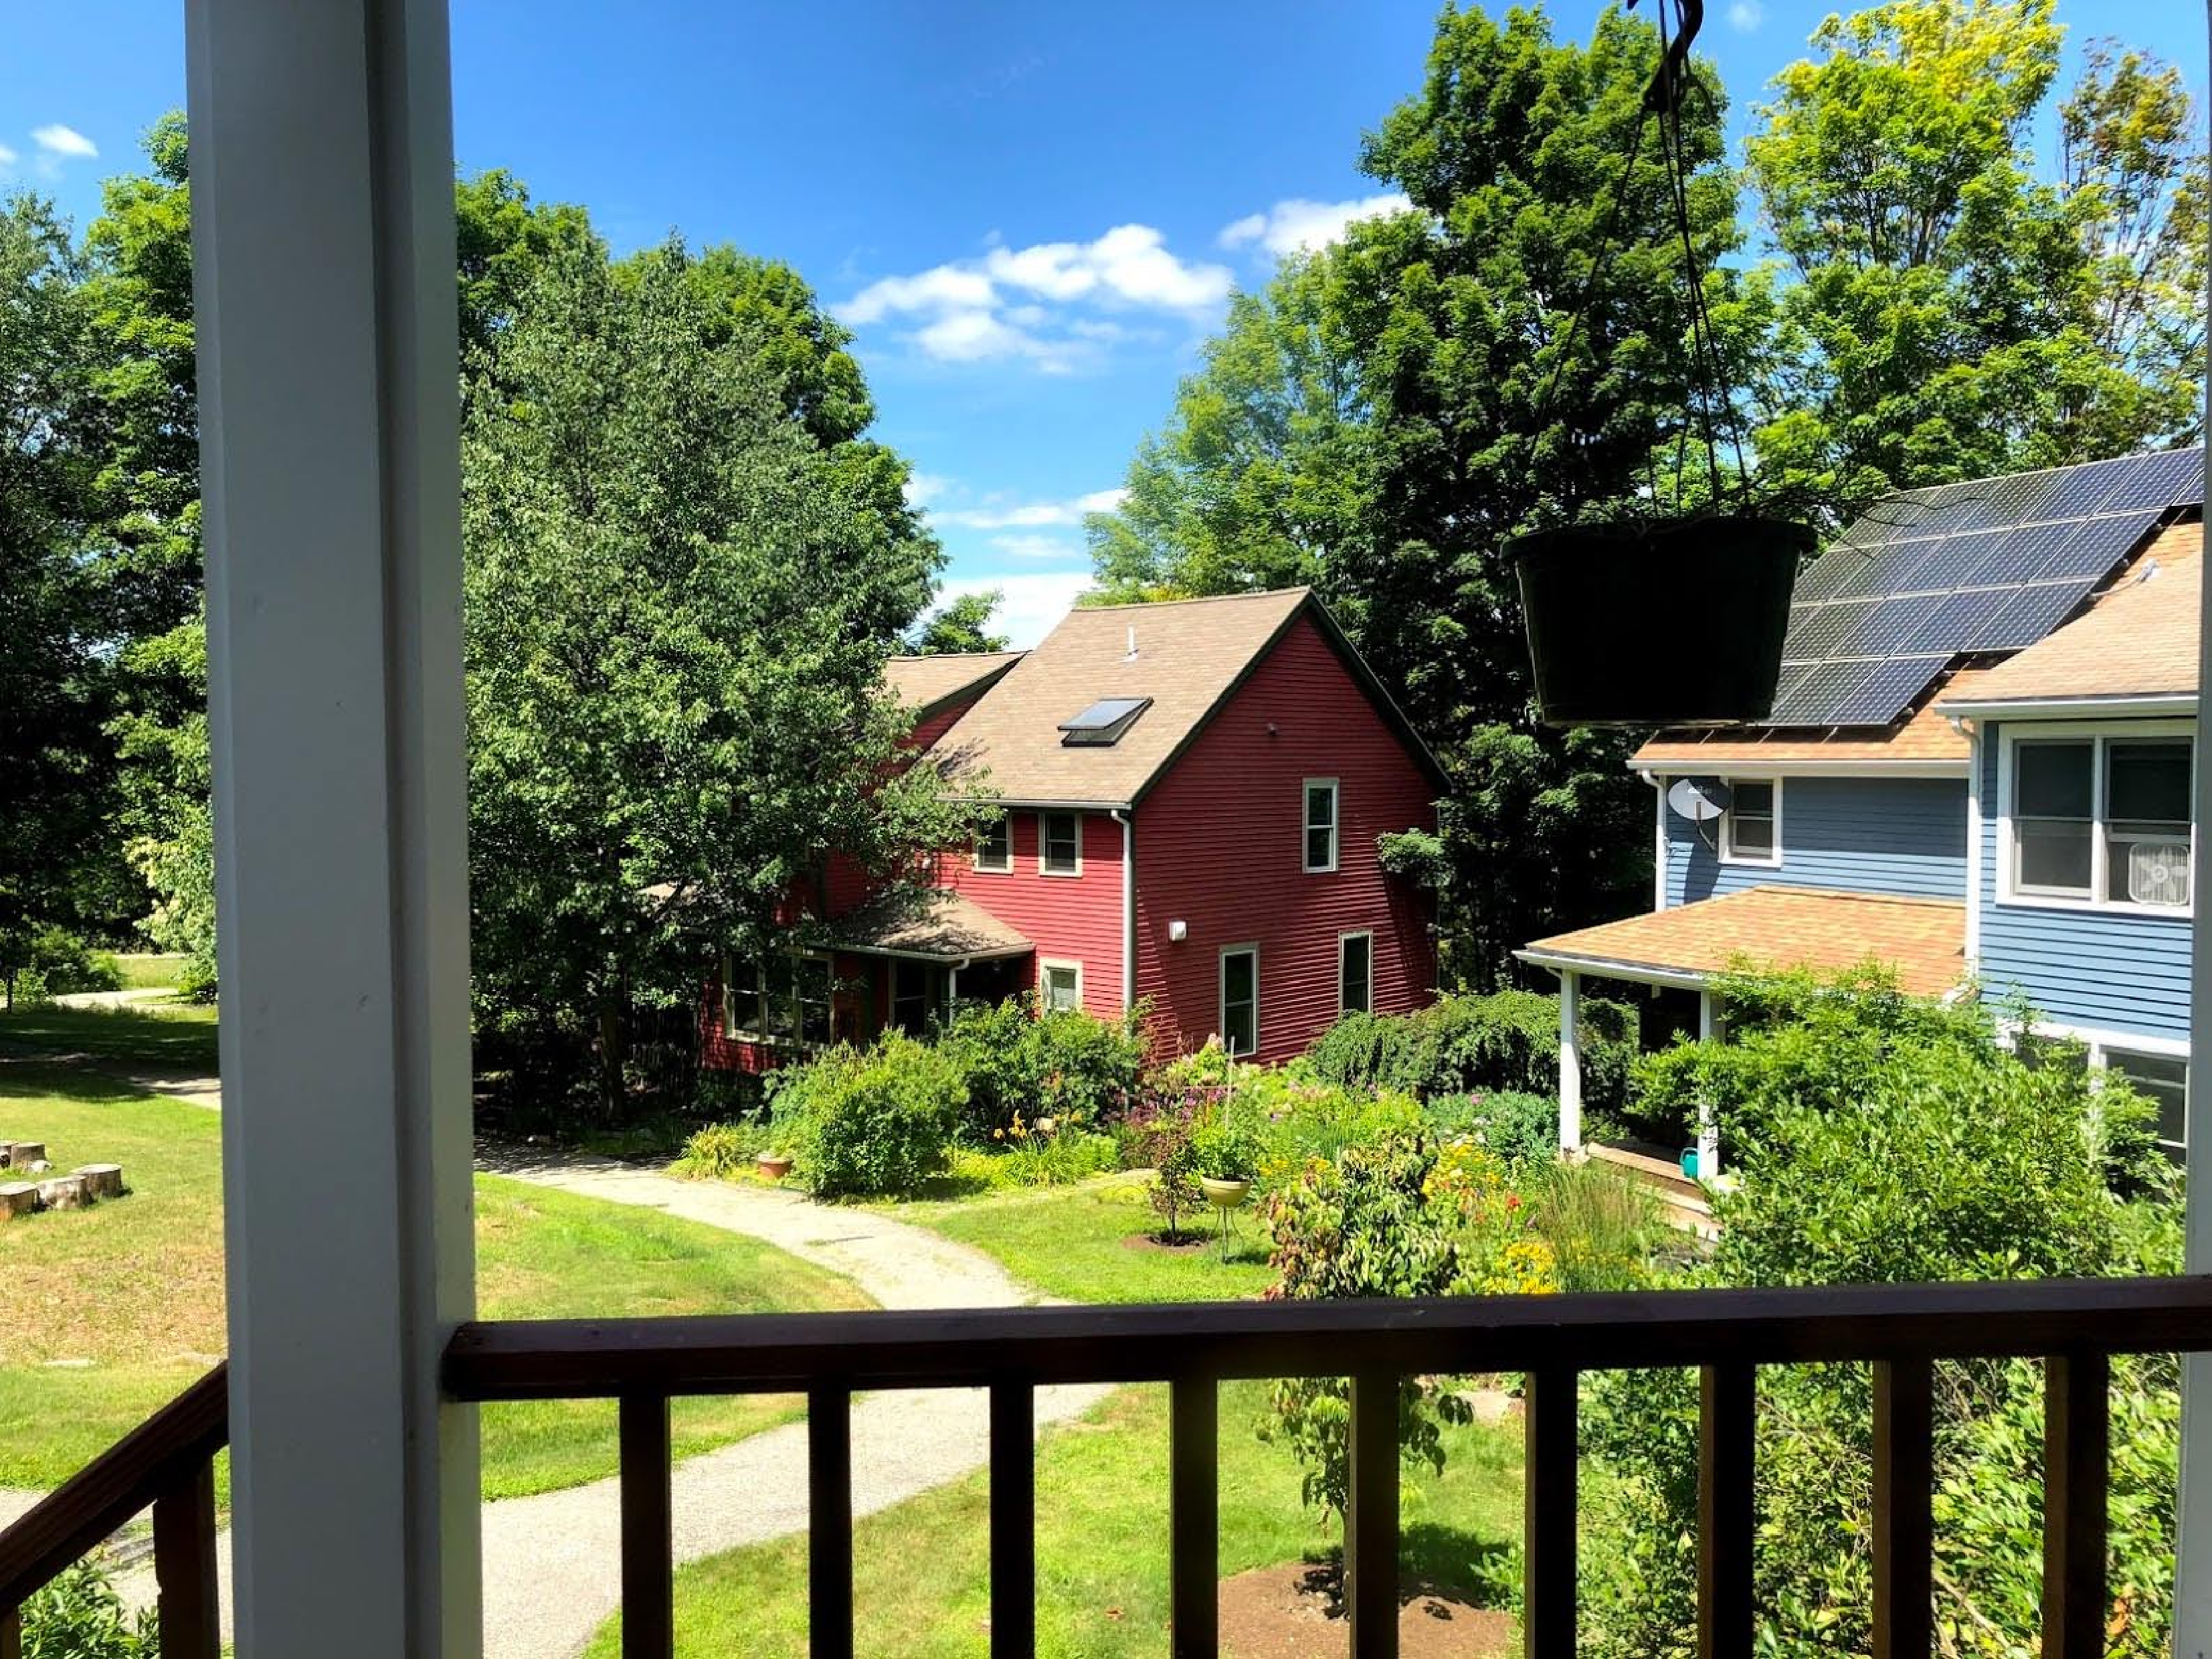
\includegraphics[width=0.5\linewidth]{figures/imaging/pinholeScene.pdf}}
%% \sublabel{b}{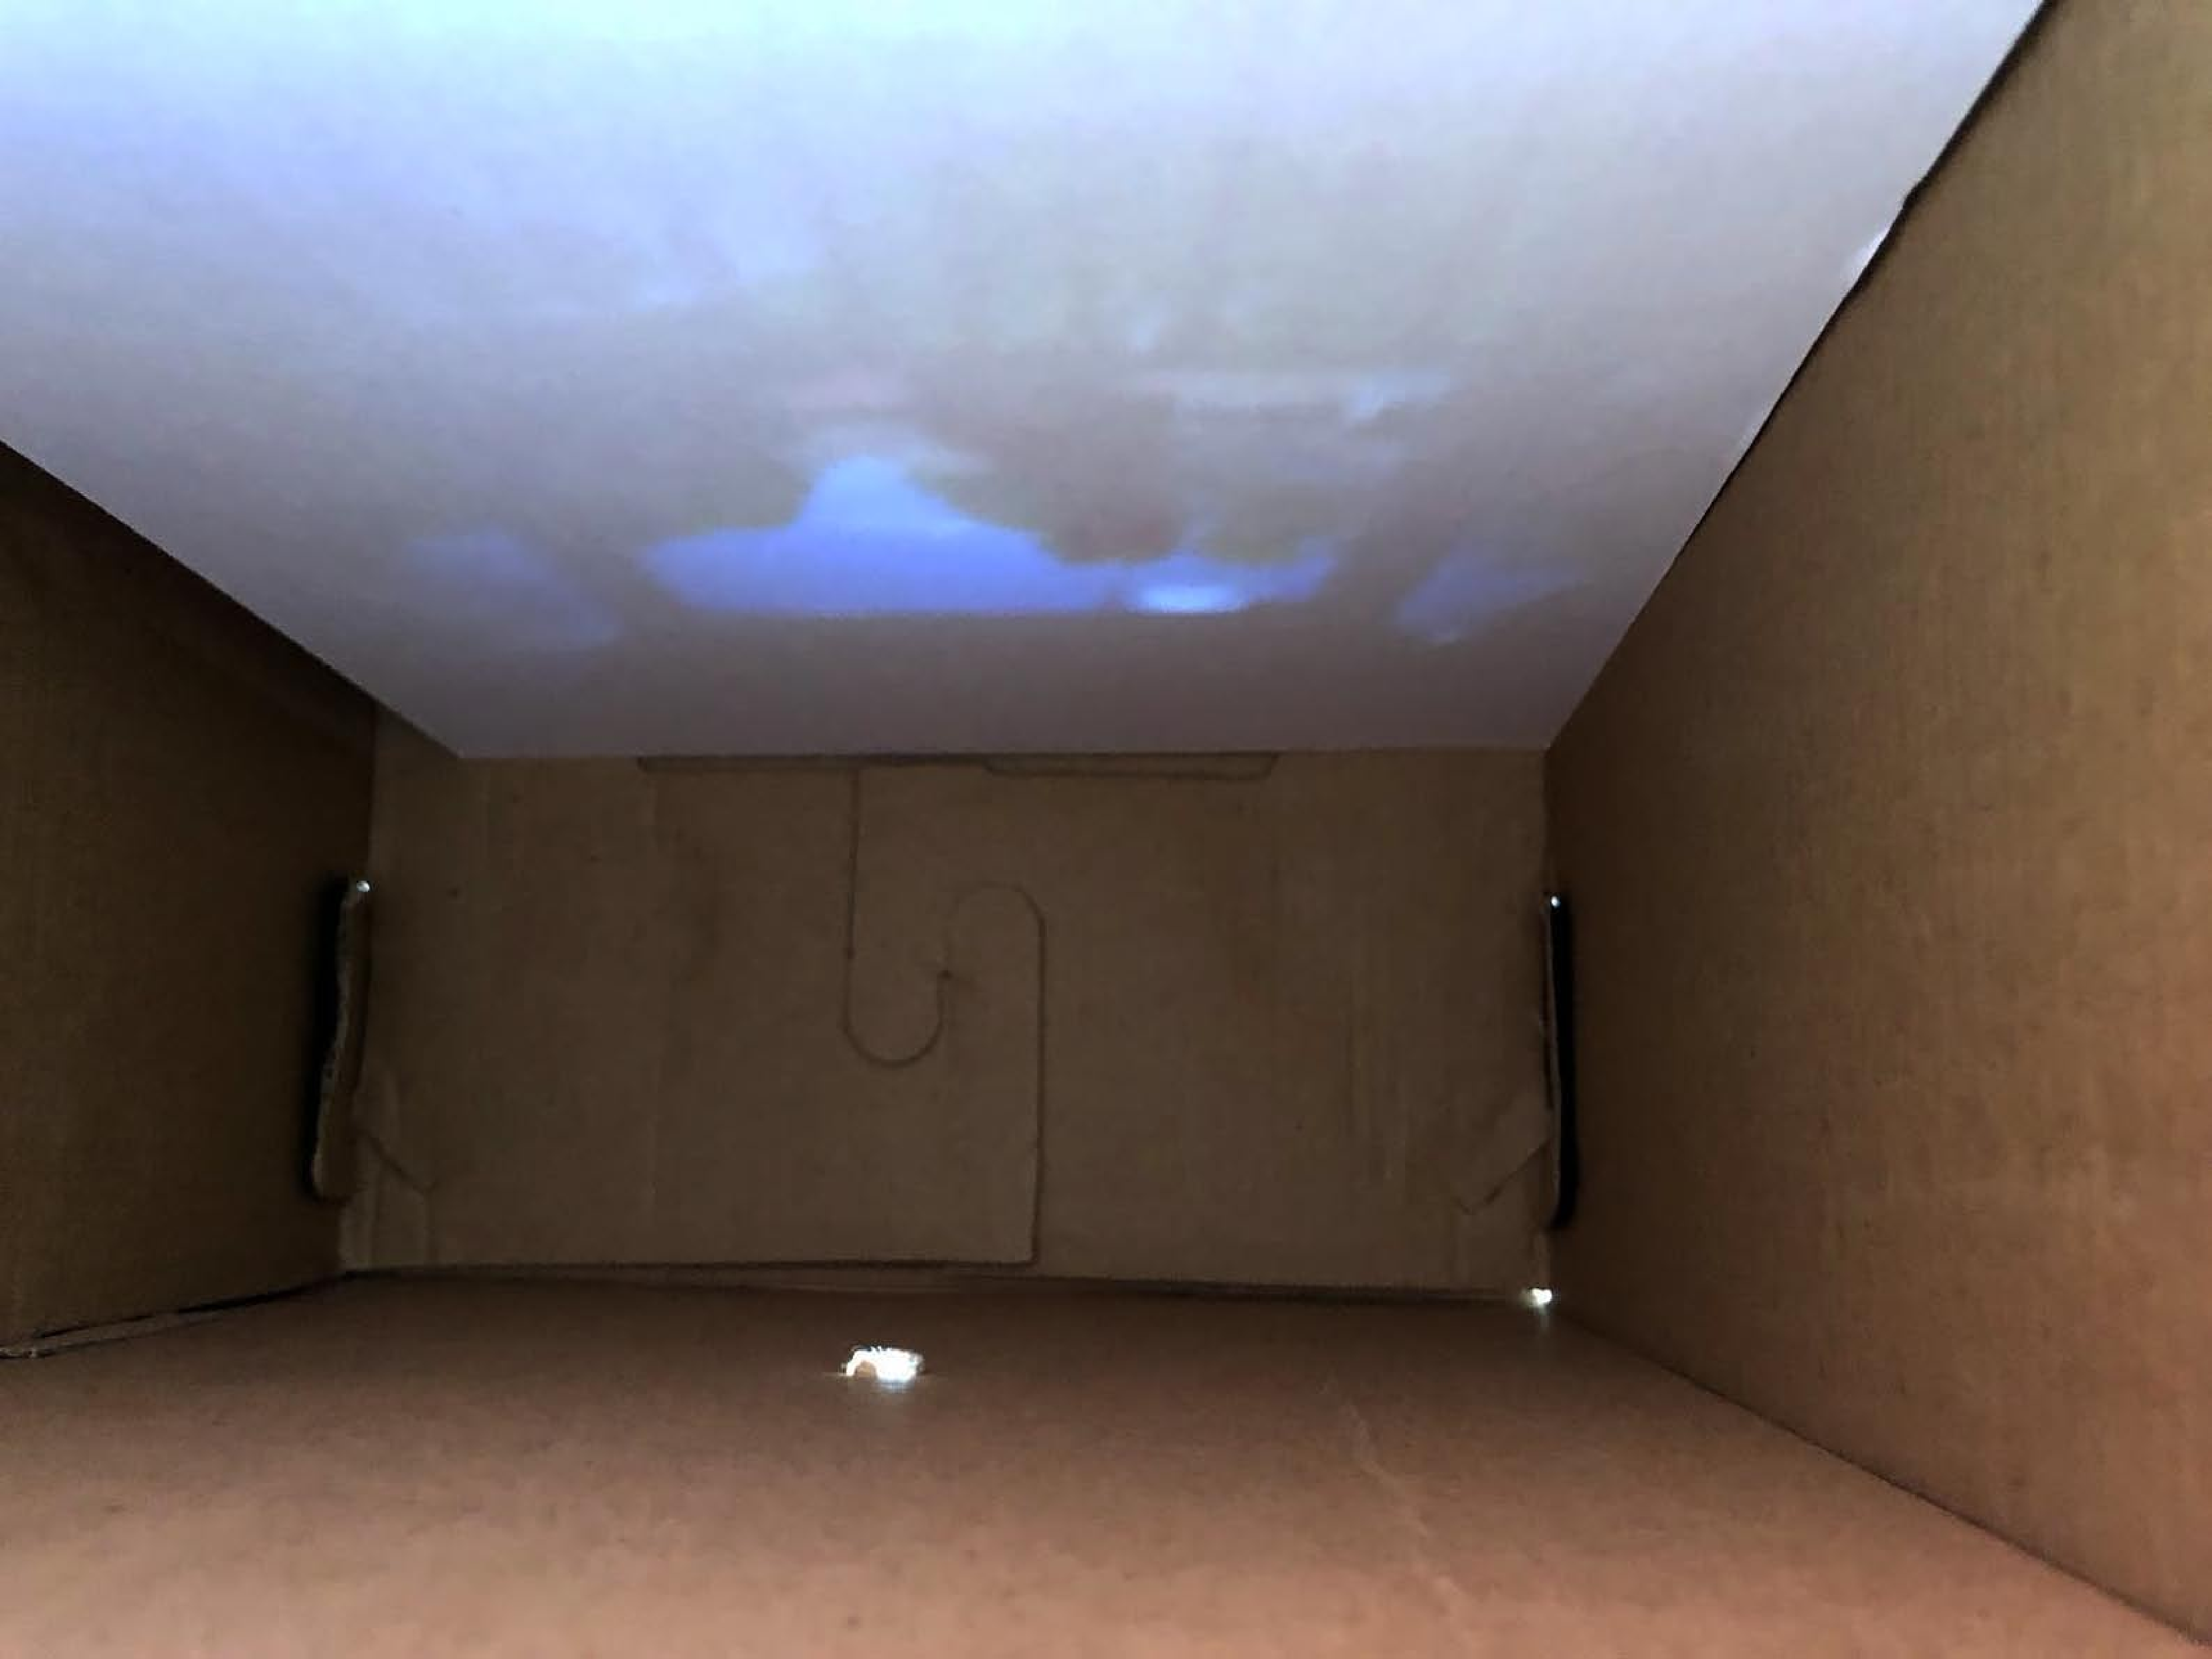
\includegraphics[width=0.5\linewidth]{figures/imaging/pinholeImage.pdf}} }


Making pinhole cameras is easy and it is a good exercise to gain an intuition of the image projection process. The picture in \fig{\ref{fig:pinhole3}} shows a very simple setup similar to the diagram from \fig{\ref{fig:wallpicture}}{b}. This setup is formed by two pieces of paper, one with a hole on it. With the right illumination conditions you can see an image projected on the white piece of paper in front of the opening. You can use this very simple setup to see the effect of changing the distance between the projection plane and the pinhole.


\begin{figure}[t]
\centerline{
\includegraphics[width=.8\linewidth]{figures/imaging/simple_pinhole.jpg}
}
\caption{A simple setting for creating images on a white piece of paper. In front of the white piece of paper we place another piece of black paper with a hole in the middle. The black paper projects a shadow on the white paper and, in the middle of the shadow, appears a picture of the scene in front of the hole. By making the hole large you will get a brighter, but blurrier image.}
\label{fig:pinhole3}
\end{figure}



\Fig{\ref{fig:pinhole2}} shows how to make a pinhole camera using a paper bag with a hole in it.  One sticks their head inside the bag, which has been padded to be opaque.
We encourage readers to make their own pinhole camera designs. The
needed elements are an aperture to let light through, mechanisms to
block stray light,  a projection screen, and some method to view or
record the image on the projection screen. 


\begin{figure}[t]
\centerline{
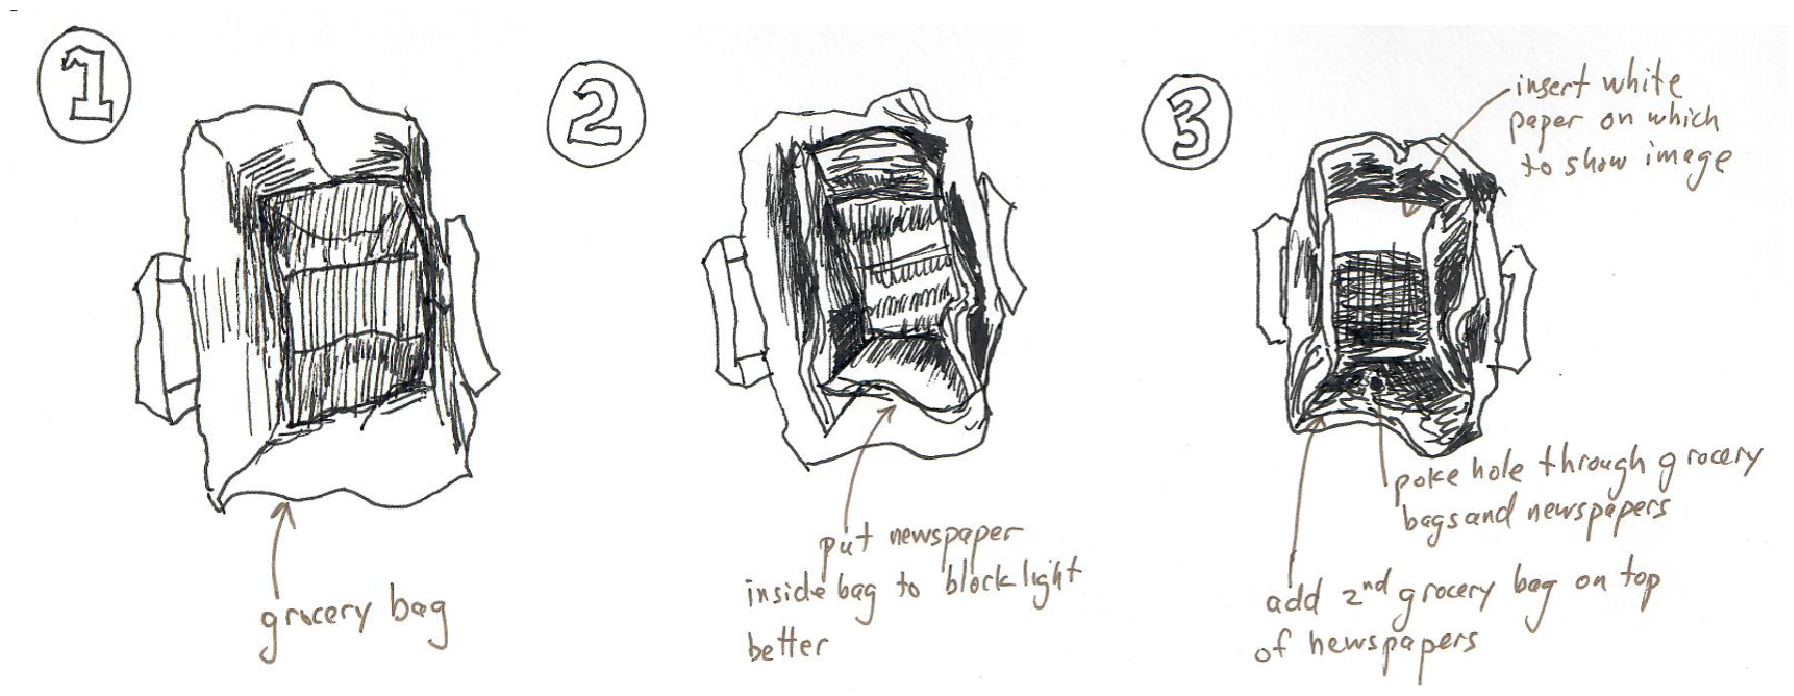
\includegraphics[width=1\linewidth]{figures/imaging/pinholeBag.pdf}
}
\centerline{
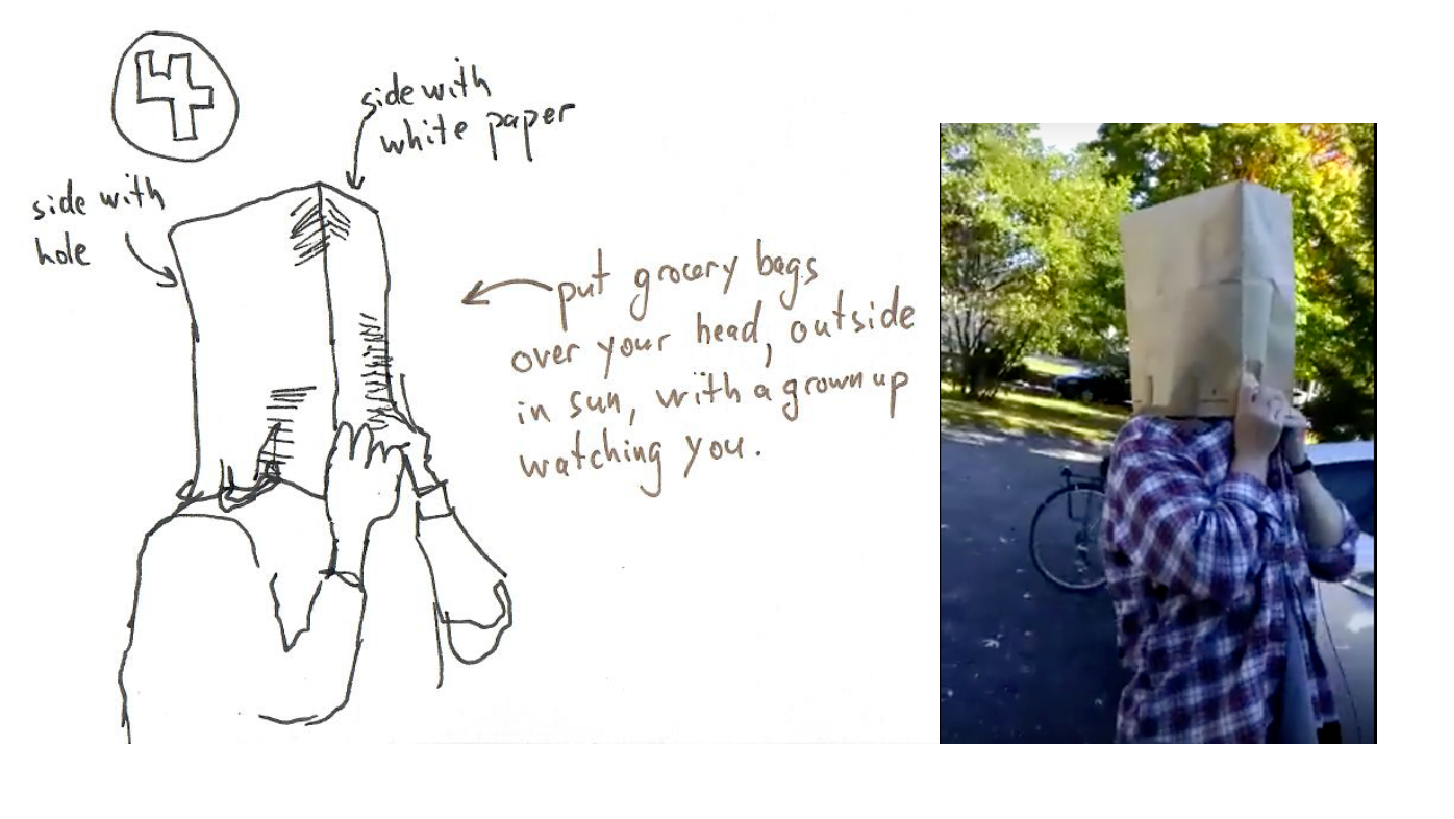
\includegraphics[width=.7\linewidth]{figures/imaging/pinholeBag2.pdf}
}
\caption{A pinhole camera made from paper bags.
Following steps 1--4, you can turn a paper bag into a light-tight pinhole camera, with the viewer inside.  Newspapers can be added between two layers of paper bags to make a light-tight enclosure. The last picture shows the use of the {\bf paper bag pinhole}
\index{Camera!Paper bag camera}
camera by one of the authors. Walking with this camera is challenging because you only get to see an upside-down version of what is behind you (adult supervision required).}
\label{fig:pinhole2}
\end{figure}


We started the section asking why there are no pictures on regular walls and explaining that, for an image to appear, we need some way of restricting the rays that hit the wall so that each location only gets rays from different directions. 
The pinhole camera is one way of forming a picture. But the reality is that, in most settings, light rays are restricted by accidental surfaces present in the space (other walls, ceiling, floor, obstacles, etc.). For instance, in a room, light rays are entering the room via a window, and therefore some of the rays are blocked. In general, the lower part of a wall will see the top of the world outside the window, while the top part of the wall will see the bottom part of the world outside the window. As a consequence, most walls will appear as having a faint blue tone on the bottom because they reflect the sky, as shown in \fig{\ref{fig:accidental}}{a}.


\begin{figure}[t]
%\centerline{
%\includegraphics[width=1\linewidth]{figures/imaging/buildingPinhole3.pdf}
%}
\centerline{
\sublabel{a}{
\includegraphics[width=.28\linewidth]{figures/imaging/room1.jpg}
}
\sublabel{b}{
\includegraphics[width=.625\linewidth]{figures/imaging/room2.jpg}
}
}
\caption{(a) A wall might contain a picture of the world after all. (b) Turning the room into a pinhole camera by closing most of the window helps to focus the picture that appears in the wall. In this case we can see some buildings that are outside the window.}
\label{fig:accidental}
\end{figure}

\marginnote{The world is full of {\bf accidental cameras}\index{Camera!Accidental camera} that create faint images often ignored by the naive observer.}

\subsection{Image Formation by Perspective Projection}

A pinhole camera projects 3D coordinates in
the world to 2D positions on the projection plane of the camera
through the straight line path of each light ray through the pinhole (\fig{\ref{fig:wallpicture}}).  The simple geometry of the camera lets us identify the projection by inspection. The sketch in \fig{\ref{fig:pinhole_names}} shows a pinhole camera and the relevant terminology. 

\begin{figure}[t]
\centerline{
\includegraphics[width=.7\linewidth]{figures/imaging/pinhole_names2.eps}
}
\caption{Coordinate systems. In computer vision it is common to use the {\bf right-hand rule} for choosing the orientation of the 3D coordinate axes.}
\label{fig:pinhole_names}
\end{figure}



\Fig{\ref{fig:pinholeGeometry}} shows the pinhole camera of \fig{\ref{fig:pinhole_names}} but with the box removed, leaving visible the projection plane. \Fig{\ref{fig:pinholeGeometry}} shows the definition of the three coordinate systems that we will use:
\begin{itemize}
    \item {\bf World coordinates}. Let the origin of a World Cartesian coordinate system be the camera's pinhole.
The coordinates of 3D position of a point, $\mathbf{P}$, in the world will be $\mathbf{P} = (X, Y, Z)$, where the Z axis is perpendicular to the
camera's sensing plane (projection plane).
    \item {\bf Camera coordinates} in the {\bf virtual camera plane}. 
    \index{Virtual camera plane}
    The camera projection plane is behind the pinhole and at a distance $f$ of the origin. Let the coordinates in the camera projection plane, $x$ and $y$, be parallel to the world coordinate axes $X$ and $Y$ but in opposite directions, respectively. For simplicity, it is useful to create a virtual camera plane that is radially symmetrical to the projection plane with respect to the origin and it is placed in front of the camera (\fig{\ref{fig:pinholeGeometry}}[a]). This virtual camera plane will create a projected image without the inversion of the image.  The coordinates in the virtual camera plane will have the same sign as the world coordinates, that is, with the same $x$,$y$ coordinates (i.e., both images are identical apart from a flip).
    \item {\bf Image coordinates}, shown in \fig{\ref{fig:pinholeGeometry}}{b}, are typically measured in pixels. Both the camera coordinate system $(x,y)$ and the image coordinate system $(n,m)$ are related by an affine transform as we will discuss later.
\end{itemize}


\begin{figure}[t]
%\centerline{
%\includegraphics[width=0.7\linewidth]{figures/imaging/pinholeGeomGumby.jpg}}
\centerline{
\includegraphics[width=1\linewidth]{figures/imaging/pinhole_geometry2.eps}
}
\caption{(a) Geometry of the pinhole camera. A 3D point $\mathbf{P}$ projects into the location $\mathbf{p}$ in the projection plane, located at a distance $f$ of the pinhole. The virtual camera plane is a radially symmetric projection of the camera plane. (b) Relation between the camera, $(x,y)$, and the image coordinate system $(n,m)$.}
\label{fig:pinholeGeometry}
\end{figure}


If the distance from the sensing plane to the pinhole is $f$ (see \fig{\ref{fig:pinholeGeometry2}})
then similar triangles
gives us the following relations:
\begin{eqnarray} 
x & = & f \frac{X}{Z} 
\label{eq:perspctiveProj1} \\
y & = & f \frac{Y}{Z} 
\label{eq:perspctiveProj}
\end{eqnarray} 
\marginnote{Thales of Miletus, 624 B.C., introduced the notion of {\bf similar triangles.}  It seems he used this to measure the height of Egypt pyramids, and the distance to boats in the sea.} 

Equations (\ref{eq:perspctiveProj1}) and (\ref{eq:perspctiveProj}) are called the {\bf perspective projection
equations}\index{Perspective projection}.  Under perspective projection, distant objects become
smaller, through the inverse scaling by $Z$.  As we will see, the perspective projection
equations apply not just to pinhole cameras but to most lens-based cameras, and
human vision as well. 



\begin{figure}[t]
\centerline{
%\includegraphics[width=.8\linewidth]{figures/imaging/pinholeGeomGumby.jpg}
\includegraphics[width=.7\linewidth]{figures/imaging/similar_triangles2.eps}
}
\caption{Perspective projection equations derived geometrically. From similar triangles, we have $x/f = X/Z$ and $y/f = Y/Z$. Similar triangles are indicated by the same color.}
\label{fig:pinholeGeometry2}
\end{figure}

Due to the choice of coordinate systems, the coordinates in the virtual camera plane have the $x$ coordinate in the opposite direction than the way we usually do for image coordinates $(m,n)$, where $m$ indexes the pixel column and $n$ the pixel row in an image. This is shown in \fig{\ref{fig:pinholeGeometry}}{b}. The relationship between camera coordinates and image coordinates is
\begin{eqnarray}
n & = & - a x + n_0\\
m & = & a y + m_0
\label{eq:cameratoimagecoordinates}
\end{eqnarray}
where $a$ is a constant, and $(n_0, m_0)$ is the image coordinates of the camera optical axis. Note that this is different than what we introduced a simple projection model in \fig{\ref{fig:projection}} in the framework of the simple vision system in \chap{\ref{chapter:simplesystem}}. In that example, we placed the world coordinate system in front of the camera, and the origin was not the location of the pinhole camera.
\marginnote{Biological systems rarely have eyes that are built as pinhole cameras. One exception is the Nautilus, which has evolved a pinhole eye (without any lens).}[-1.2in]


\subsection{Image Formation by Orthographic Projection}

Perspective projection is not the only feasible projection from 3D
coordinates of a scene
down to the 2D coordinates of the sensor plane.  Different camera geometries can lead to other projections.  One alternative to perspective projection is {\bf orthographic projection}\index{Orthographic projection}. \Fig{\ref{fig:orthographics}} shows the geometric interpretation of orthographic (or parallel) projection. 


\begin{figure}[t]
\centerline{
%\includegraphics[width=.8\linewidth]{figures/imaging/pinholeGeomGumby.jpg}
\includegraphics[width=.9\linewidth]{figures/imaging/orthogonal_projection.eps}
}
\caption{Orthographic projection. Projection is done by parallel rays orthogonal to the projection plane. In this example, we have $x = X$ and $y = Y$.}
\label{fig:orthographics}
\end{figure}

In this projection, as the rays are orthogonal to the projection plane, the size of
objects is independent of the distance to the camera. The projection equations are generally written as follows:
\begin{eqnarray}
x & = & k X \nonumber \\
y & = & k Y
\label{eq:orthographicProj}
\end{eqnarray}
where the constant scaling factor $k$ accounts for change of units and is a fixed global image scaling.

Orthographic projection is a good model for telephoto lenses, where the apparent size of objects in the image
is roughly independent of their distance to the camera.  
We used this projection when building the simple visual system in \chap{\ref{chapter:simplesystem}}.


\marginnote{Orthographic Projection is a correct model when looking at an infinitely far away object that is infinitely zoomed in, as discussed in \chap{\ref{chapter:simplesystem}}.}

The next section provides another example of a camera producing an orthographic projection. 


\subsection{How to Build an Orthographic Camera?}
\index{Camera!Orthographic camera}

Can we build a camera that has an orthographic projection? What we need is some way of restricting the light rays so that only perpendicular rays to the plane illuminate the projection plane.

One such camera is the {\bf soda straw camera}\index{Camera!Soda straw camera}, shown in \fig{\ref{fig:straw}}, which you can easily build. The example shown in (c) used around 500 straws.  



\begin{figure}
\centerline{
\includegraphics[width=1\linewidth]{figures/imaging/straw_camera.eps}
}
\caption{Straw camera example.  (a) View through parallel straws. (b) The subject is  a hand in sunlight.  (c)
The resulting image of the straw camera (using smaller straws than (a)).  The image projection is orthographic.}
\label{fig:straw}
\end{figure}


A set
of parallel straws allow parallel light rays to pass from the scene to
the projection plane, but extinguish rays passing from all other
directions. It works better if the straws are painted black to reduce internal reflections that might capture light rays not parallel to the straws, resulting in a less sharp picture. 


\Fig{\ref{fig:straw}}{c} shows the resulting image when imagining the scene shown in \fig{\ref{fig:straw}}{b}. The straw camera doesn't invert the image as the pinhole camera does and objects do not get smaller as they move away from the camera. The image projection is orthographic, with a unity scale factor; the object sizes on the projection plane are the same as those of the objects in the world.

% http://strawcamera.com/

\marginnote{A larger straw camera has been built by Michael Farrell and Cliff Haynes \cite{straw2017} with an impressive 32,000 drinking straws.}


Another implementation of an orthographic camera is the telecentric lens that combines a pinhole with a lens. 
%\marginnote{Maybe the fly's eye is somewhat similar to the straw camera?}

%\centerline{
%\sublabelnp{(a) View through straws of straw camera}
%{\includegraphics[width=0.25\linewidth]{figures/imaging/strawElements.jpg}}
%\sublabelnp{(b) outside of straw camera}{\includegraphics[width=0.4\linewidth]{figures/imaging/strawSceneFocus.pdf}}
%\sublabelnp{(c) \href{https://groups.csail.mit.edu/vision/cvbook/videos/IMG_2948.MOV}{video of straw camera projection.}}{\includegraphics[width=0.3\linewidth]{figures/imaging/strawImageContrast.pdf}}}

%% INTRODUCE THIS SOMEWHERE ELSE
%% \subsubsection{Homogeneous coordinates}
%% 
%% The projection matrix for coordinate %% values, r = MR.

\section{Concluding Remarks}

Light reflects off surfaces and scatters in many directions.  Pinhole cameras allow only selected rays to pass to a sensing plane, resulting in a perspective projection of the 3D scene onto the sensor.  Other camera configurations can give other image projections, such as orthographic projections.

At this point, it is a good exercise to build your own pinhole camera and experiment with it. Building a pinhole camera helps in acquiring a better intuition about the image formation process. 




%%%%%%%%%%%%%%%%%%%%%%%%%%%%%%%%%%%%%%%%%%%%%%%%%%%%%%%
\chapter{Lenses}
\label{chapter:lenses}


%\section{Lenses}

\section{Introduction}

While pinhole cameras can form good images, they suffer from a serious drawback:  the images are very dim because not much light passes through the small pinhole to the sensing plane of the pinhole camera. As shown in figures \ref{fig:pinholes} and \ref{fig:pinholeSize}, one can try to let in more light by making the pinhole aperture bigger.  But that allows light from many different positions to land on a given position at the sensor plane, resulting in a bright but blurry image.  Putting a lens in the larger aperture can give the best of both worlds,  capturing more light while redirecting the light rays entering the camera so that each sensor plane position maps to just one surface point, creating a focused image on the sensor plane.  Here we analyze how light passes through lenses under the approximation of {\bf geometric optics}\index{Geometric optics}, where we ignore effects like diffraction, due to the wave nature of light.



\begin{figure}[h!]
\centerline{
\includegraphics[width=.9\linewidth]{figures/imaging/apertures_and_lenses.pdf}
}
%\centerline{
%\sublabelnp{(a) Image from small pinhole}{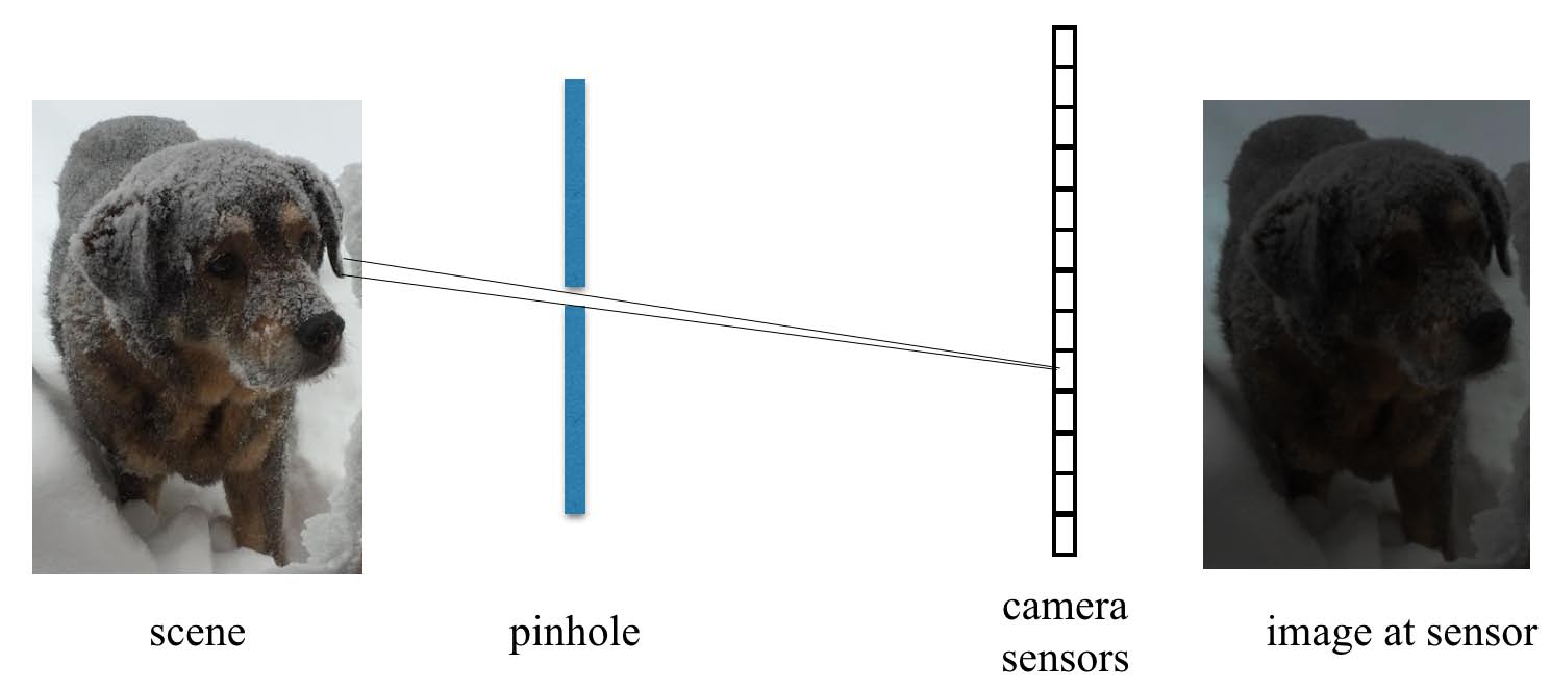
\includegraphics[width=0.7\linewidth]{figures/imaging/toby1.pdf}}}
%\centerline{
%\sublabelnp{(b) Image from large pinhole}{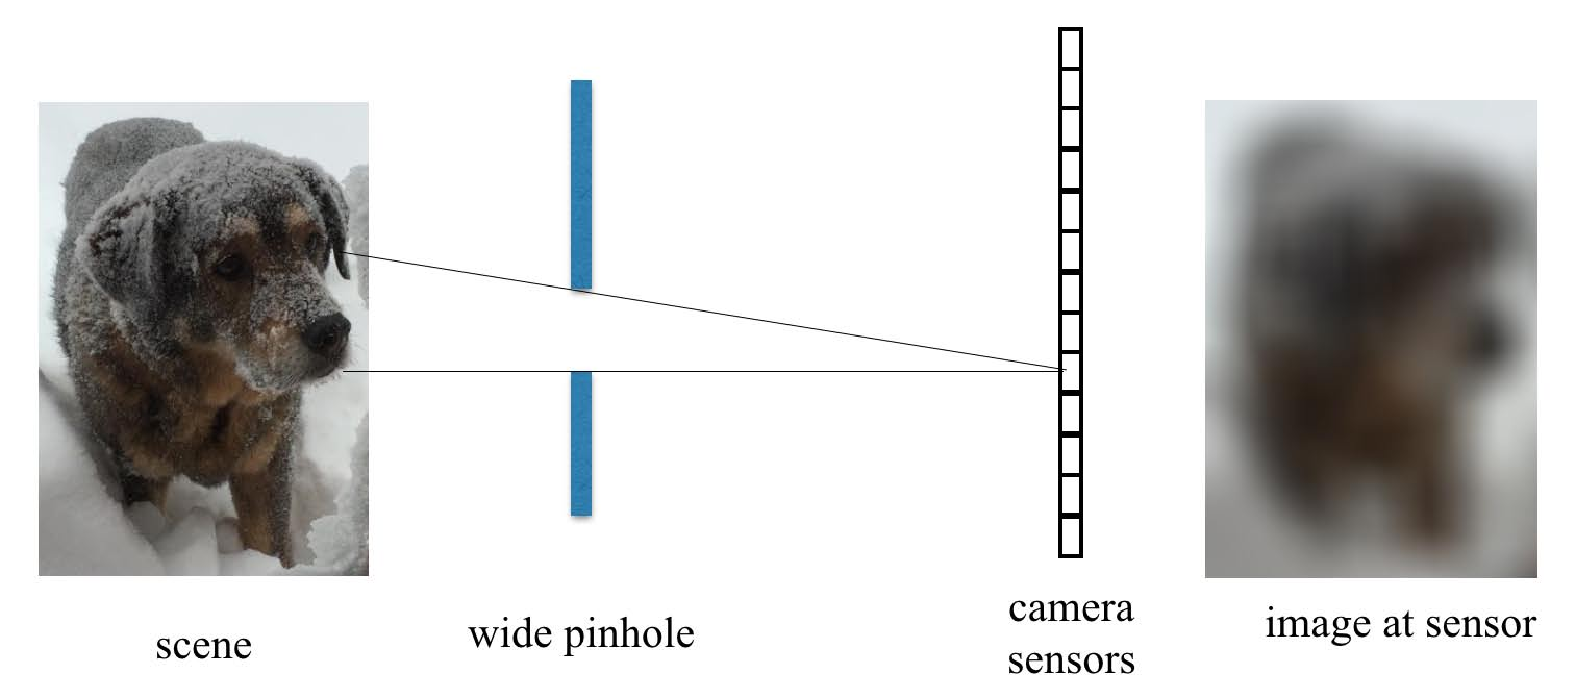
\includegraphics[width=0.7\linewidth]{figures/imaging/toby2.pdf}}}
%\centerline{
%\sublabelnp{(c) Image from lens within the large pinhole}{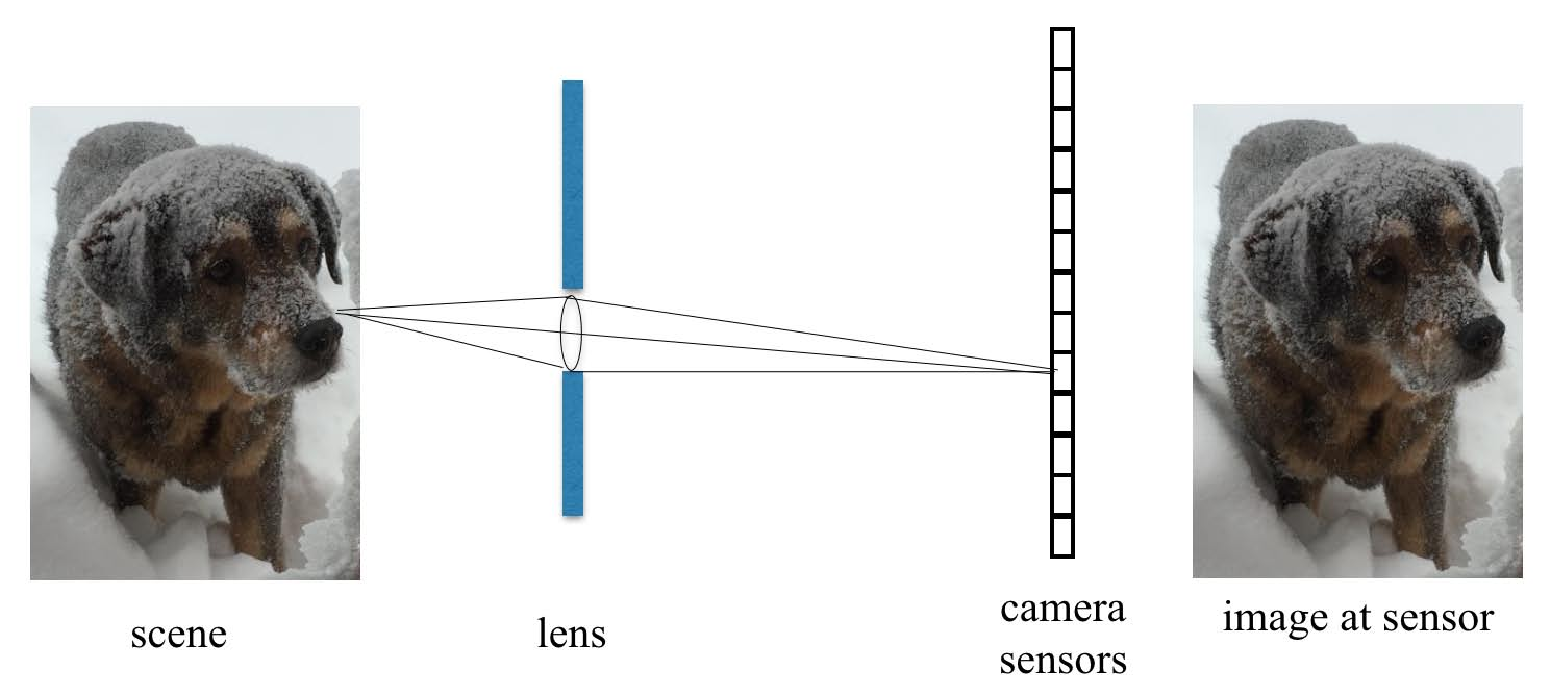
\includegraphics[width=0.7\linewidth]{figures/imaging/toby3.pdf}}}
\caption{Brightness/sharpness trade-offs in image formation. From left to right a small pinhole will create a sharp image, but lets in little light, so the image may appear dark for a given exposure time. A larger pinhole lets in more light and generates a brighter image, but each sensor element records light from many different image positions, creating a blurry image. A lens can collect light reflected over many different angles from a single point, allowing a bright, sharp image.}
\label{fig:pinholes}
\end{figure}


\begin{figure}
\centerline{
\includegraphics[width=1\linewidth]{figures/imaging/gumbyEdited.jpg}
}
%\centerline{
%\sublabel{a}{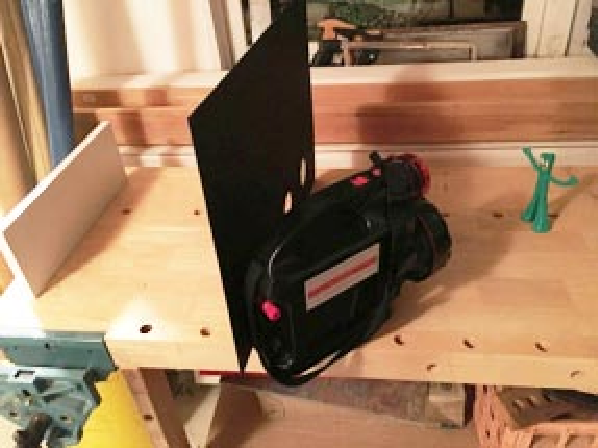
\includegraphics[width=0.5\linewidth]{figures/imaging/pinhole3.pdf}}}
%\centerline{
%\sublabel{b}{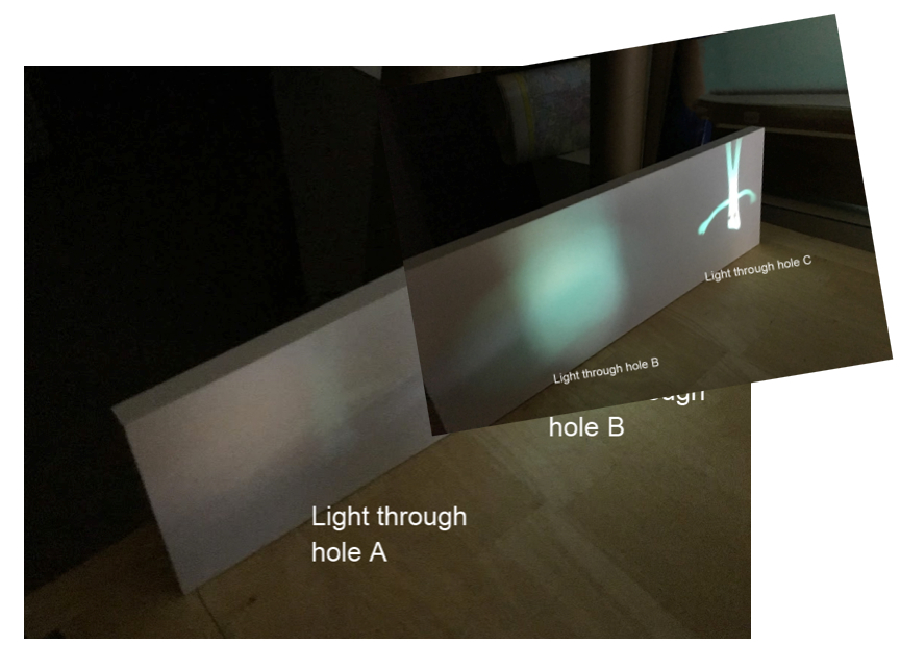
\includegraphics[width=0.45\linewidth]{figures/imaging/tmpGumbys.pdf}}
%\sublabel{c}{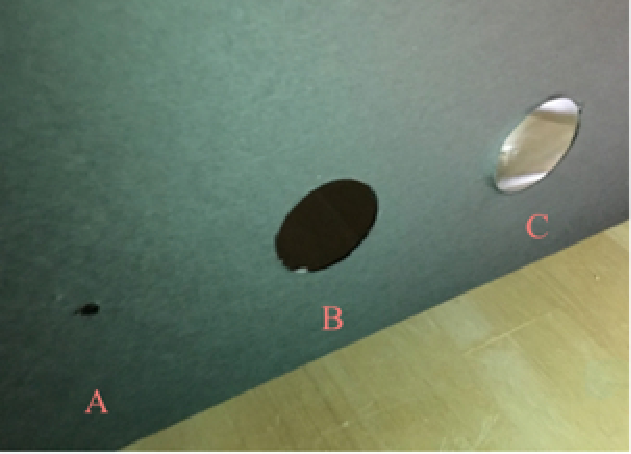
\includegraphics[width=0.4\linewidth]{figures/imaging/pinhole4.pdf}}
%\sublabel{d}{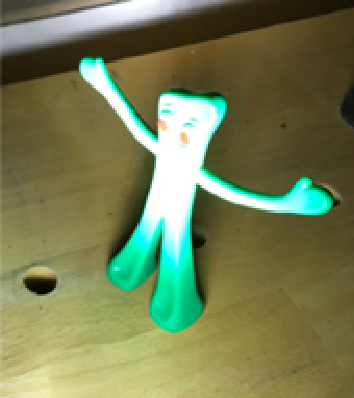
\includegraphics[width=0.3\linewidth]{figures/imaging/gumby.pdf}}}
\caption{Physical demonstration of the trade-offs illustrated in \fig{\ref{fig:pinholes}}. (a) Gumby subject, illumination light,
  barrier with the three apertures, and white projection screen. Also, a light source is added to illuminate the subject. (b) Picture of Gumby. (c)
  Images formed by light through the three apertures. (d) Detail of the three
  apertures (small pinhole, large pinhole, and lens).}
\label{fig:pinholeSize}
\end{figure}




\section{Lensmaker's Formula}
\label{sect:lensmaker}

In general, light changes both its wavelength and its speed as it passes from one material to another.  Those changes at the material interface
will cause the light to bend, an effect called {\bf refraction}\index{Refraction}.  The amount of light bending depends on the change of speed of light within each material, and the orientation of the light ray with respect to the interface surface, according to {\bf Snell's Law}\index{Snell's Law} \cite{Hecht2016}, given in the equation below.  Both the wavelength and the speed of light in a medium are inversely proportional to the {\bf index of refraction}\index{Index of refraction} of that medium, denoted as $n$.  The $n$ for a vacuum is 1.  At a material boundary, for the geometry illustrated in \fig{\ref{fig:snell}}, we have
\begin{equation}
n_1 \sin(\theta_1) = n_2 \sin(\theta_2)
\end{equation}
where $\theta_1$ and  $\theta_2$ are the angles with respect to the surface normal of the incident and outgoing light rays, and $n_1$ and $n_2$ are the  indices of refraction of the materials in region 1 and region 2. Snell's law can be derived by matching the wavelength of light projected along the material interface boundary across each side of the boundary.

\marginnote{Snell's Law relates the bending angles of refraction, $\theta_1$ and $\theta_2$, to the indices of refraction, $n_1$ and $n_2$, at a material interface.}

\begin{figure}
\centerline{
%%\sublabel{a}{\includegraphics[width=0.42\linewidth]{figures/imaging/snell.jpg}}
\sublabel{a}{\includegraphics[width=0.40\linewidth]{figures/imaging/snellcropped.eps}}
\sublabel{b}{\includegraphics[width=0.53\linewidth]{figures/imaging/IMG_2490.JPG}}
}
\caption{(a) Snell's law describes the bending of light at interfaces of differing indices of refraction, $n_1$ and $n_2$, in terms of the angles, $\theta_1$ and $\theta_2$, relative to the interface, or surface, normal. (b) Straw below water surface appears distorted due to refraction at the air/water boundary. Note that (a) and (b) are not trivially connected!}
\label{fig:snell}
\end{figure}


A lens is a specially shaped piece of transparent material, positioned to focus light from a surface point onto a sensor. In an ideal world, a lens focusing light from a surface onto a sensor plane has the property that every light ray from the surface point that passes through the lens is refracted onto a common position at the sensor, no matter what part of the lens the ray from the surface hits.  This dramatically increases the light-gathering ability of the camera system, overcoming the poor light-gathering properties of a pinhole camera system.

To achieve that property, we must find a surface shape that allows for this focusing.
Modern lens surfaces are designed by numerical optimization methods, trading off engineering constraints to achieve the best design, often involving several optical elements and different materials.  But to gain insight into the properties of lenses, we can analytically design a lens surface shape provided we simplify the optical system.

For small angles $\theta$ denoted in radians, $\sin(\theta) \approx \theta$.  If we also assume the index of refraction of air is 1 (it is 1.0003) and denote the index of refraction of lens glass as $n$, then Snell's law, as shown in \fig{\ref{fig:snell}}, becomes
%\marginnote{Snell's law for small angles $\theta_1$ and $\theta_2$.}[.1in]
\begin{equation}
\theta_1 = n \theta_2,    
\end{equation}
for small bending angles $\theta_1$ and $\theta_2$.



Consider a lens, and two points along its optical axis at a distance $a$ and $b$ from the lens, as shown in \fig{\ref{fig:lens}}{a}.
We seek to find a surface shape for a lens which creates the light paths shown in \fig{\ref{fig:lens}}{a}:  light leaving from any direction at point $a$ will be focused to arrive at point $b$.  \Fig{\ref{fig:lens}}{b} shows a view of \fig{\ref{fig:lens}}(a), with angles and distances distorted for clarity of labeling.

\begin{figure}
\centerline{
\sublabel{a}{\includegraphics[width=0.9\linewidth]{figures/imaging/lensRealCropped.pdf}}}
\centerline{
\sublabel{b}{\includegraphics[width=1.0\linewidth]{figures/imaging/lensDistortedCropped.pdf}}}
%% \centerline{
%% \sublabel{c}{\includegraphics[width=0.7\linewidth]{figures/imaging/lensSurface.jpg}}}
\caption{(a) The geometry of a thin lens. (b) Showing the labels of adding angles referenced in table~\ref{tab:lensmaker}, used to describe the conditions for the lens shape, $\theta_S$ to give the desired focusing. Geometry  is distorted for visibility.}
\label{fig:lens}
\end{figure}
% see perspective.key from Bill's laptop dropbox for the keynote source figures


We make use of several approximations that commonly hold for imaging systems: the deviations in angle from the optical axes are very small (i.e., the {\em paraxial approximation}) and the lens is modeled to have negligible thickness compared with other distances along the optical axis (i.e., the {\em thin lens approximation}\index{Lens!thin}).  Under those approximations, we can write simple expressions for the bending angles shown in \fig{\ref{fig:lens}}{b} as a function of $\theta_S$,  the lens surface orientation at height $c$.  Those relations are summarized below in table~\ref{tab:lensmaker}.

The middle row of table~\ref{tab:lensmaker} requires explanation.  The light ray within the lens, depicted in \fig{\ref{fig:lens}}{b}, is not necessarily parallel to the optical axis.  In general, it will be rotated by some angle $\delta$ away from the optical axis, giving $\theta_S = \theta_2 + \delta$, and, at the other lens surface, $\theta_S = \theta_3 - \delta$.  Adding those two equations removes $\delta$ and gives the relation $2 \theta_s = \theta_2 + \theta_3$


\begin{table}
%\marginnote{{\bf Table \ref{tab:lensmaker}}: Relations between angles of thin lens example, \fig{\ref{fig:lens}}{b}} % Hack to get the caption of the table in the margin.
\caption{Relations between angles of thin lens example, \fig{\ref{fig:lens}}{b}}
%\faketablecaption{}
\begin{center}
\begin{tabular}{| c c c c |}
\hline
{\bf Angle}  & {\bf Description} & {\bf Relation} & {\bf Reason} \\
\hline
 $\theta_1 $ &
 Initial angle from optical axis & $\theta_1 = c/a$ & Small angle approx.\\ 
  \hline
  & 
 Angle of refracted ray & & Snell's law, \\ 
  $\theta_2$ & wrt front surface normal & $n \theta_2 = \theta_1 + \theta_S$   & small angle approx. \\ 
 \hline
 &
 Angle of refracted ray & & Symmetry of lens,\\ 
  $\theta_3$ & wrt back surface normal & $2 \theta_S  = \theta_2 + \theta_3$  & thin lens approx.\\ 
 \hline
&
 Angle of ray exiting lens & & Snell's law, \\ 
  $\theta_4 + \theta_S$ & wrt back surface normal & $n \theta_3 = \theta_4+\theta_S$  & small angle approx.\\
 \hline
 $\theta_4$ &
  Final angle from optical axis & $\theta_4 = c/b$ & Small angle approx. \\
  \hline 
\end{tabular}
\end{center}
\label{tab:lensmaker}
\end{table}

If we start from the relation in table~\ref{tab:lensmaker} for $\theta_4$, and substitute for each angle using the relation in each line above, up through $\theta_1 = c/a$, we can algebraically eliminate the angles $\theta_1$ through $\theta_4$ to find the condition on the lens surface angle, $\theta_S$, as a function of the distance $c$ from the optical axis, which  allows for the desired focusing to occur.  The result is as follows: 
\begin{equation}
    \theta_S = \frac{c}{2(n-1)} \left( \frac{1}{a} + \frac{1}{b} \right)
\label{eq:ts1}
\end{equation}
This relationship creates the effect that every ray emanating at a small angle from point $a$ will be focused to point $b$.  \Eqn{\ref{eq:ts1}} shows that the lens surface angle, $\theta_S$, must deviate from flat in linear proportional to the distance $c$ from the center of the lens.

\marginnote{To focus, the lens surface angle, $\theta_S$, must be a {\em linear} function of the distance, $c$, from the center of the lens.}[-.3in]

%\begin{figure}
%\centerline{
%\includegraphics[width=0.3\linewidth]{figures/imaging/sphereLens3.pdf}}
%\caption{Relation between $R$ and $\theta_S$, in \eqn{\ref{eq:ts2}}, for a spherical lens.}
%\label{fig:sphereLens}
%\end{figure}

In the thin lens approximation, both parabolic and spherical shapes satisfy that constraint on the lens surface slope.
For a spherical lens surface, such as \fig{\ref{fig:sphereLens}},  curving according to a radius $R$, we have $\sin(\theta_S) = c/R$.  For small angles $\theta_S$, this reduces to
\begin{equation}
    \theta_S = \frac{c}{R},
    \label{eq:ts2}
\end{equation}
where $R$ is the radius of the sphere, which has the desired property that $\theta_S \propto c$.  


\begin{figure}
\centerline{
\includegraphics[width=0.3\linewidth]{figures/imaging/sphereLens3.pdf}}
\caption{Relation between $R$ and $\theta_S$, in \eqn{\ref{eq:ts2}}, for a spherical lens.}
\label{fig:sphereLens}
\end{figure}

Substituting \eqn{\ref{eq:ts2}} into the focusing condition, 
\eqn{\ref{eq:ts1}} yields the {\bf Lensmaker's Formula}\index{Lensmaker's Formula},
\begin{equation}
\frac{1}{a} + \frac{1}{b} = \frac{1}{f},
\label{eq:lensmaker}
\end{equation}
where the lens {\bf focal length}\index{Focal length}, $f$ is defined to be
\begin{equation}
    f = \frac{R}{2(n-1)}
\end{equation}

It is straightforward to show, by rotating the lens in \fig{\ref{fig:lens}}{a} through an angle $\theta_R$ in the above derivation, thus adding $\theta_R$ to $\theta_S$ in table~\ref{tab:lensmaker},
that the lensmaker's equation also holds for light originating off the optical axis.   Thus, under the paraxial and thin lens approximations, the lens focuses light from points on a plane onto points on a second plane, both perpendicular to the optical axis, as illustrated in \fig{\ref{fig:rotatedLens}}.


\begin{figure}
\centerline{
\includegraphics[width=1\linewidth]{figures/imaging/offAxis.pdf}}
\caption{Considering light from off-axis sources is equivalent to rotating the lens surface by $\theta_R$, for small angles $\theta_R$.  The lens focuses rays from off-axis points like $P_1$, as well as from the on-axis point, $P_0$.}
\label{fig:rotatedLens}
\end{figure}


One can also generalize the equation for the case of a lens with different radii of curvature, $R_1$ and $R_2$ on the front and back faces of the lens.  Defining the left and right surface angles $\theta_{s_1}$ and $\theta_{s_2}$, respectively, the middle row equation of table~\ref{tab:lensmaker} becomes $\theta_{s_1} + \theta_{s_2} = \theta_2 + \theta_3$.  Then, the equation substitutions of Table~\ref{tab:lensmaker}, combined with $\theta_{S_i} = c / R_i$, for $i = 1$ and $2$,
lead to
\begin{equation}
    \frac{1}{f} = (n-1) \left( \frac{1}{R_1} + \frac{1}{R_2} \right)
\end{equation}
Note that some texts (e.g., \cite{Hecht2016}) adopt a sign convention where the back surface of a lens is defined to have negative curvature.


\Fig{\ref{fig:greenLaser}} shows a demonstration of the focusing
property for a thin lens. % of a 20cm focal length.  
The hand, labeled (a), is flicking a laser pointer back and forth,
sending light rays in many directions from a central point during the image exposure, as would a diffuse surface reflection.  All the light rays that strike the lens, labeled (b), are focused to the same green spot, labeled (c), while the light rays passing  outside the lens at (b) reveal their straight line trajectories on the wall at (c).


\begin{figure}
\centerline{
\includegraphics[width=0.6\linewidth]{figures/imaging/greenLaserBrightenedCrop2.jpg}
}
\caption{Demonstration showing that a lens focuses a fan of rays, such as those reflecting from a diffuse surface, to a point.  (a) Here the right hand wiggles a laser pointer back and forth during the photographic exposure, generating a fan of light rays, approximating (in one dimension) rays reflecting from one point on a diffuse surface.   (b) The fan of rays sweeps across a lens, which focuses each ray passing through the lens to the same spot at the wall, (c), regardless of where each ray had entered the lens.  (c) The rays that pass outside the lens form the two line segments on either side.}
\label{fig:greenLaser}
\end{figure}
\clearpage % Avoid using clearpage command 

\section{Imaging with Lenses}
\label{sect:imagingWithLenses}

Armed with the lensmaker's formula and the observation of \fig{\ref{fig:thinLens}}, we can analyze how rays travel through lenses in the approximation of geometrical optics. Light passing through the center of a thin lens, where the front and back surfaces are parallel, proceeds without bending.  Thus a convex thin lens\index{Lens!convex} images as a pinhole camera does, creating a perspective projection.
\begin{figure}
\centerline{
\sublabel{a}{\includegraphics[width=0.25\linewidth]{figures/imaging/centerThick.pdf}}
\sublabel{b}{\includegraphics[width=0.25\linewidth]{figures/imaging/centerThin.pdf}}
\sublabel{c}{\includegraphics[width=0.46\linewidth]{figures/imaging/lenspinhole3.pdf}}
}
\caption{Light travels straight through the center of a thin lens, where front and back surfaces are parallel.  (a) Lens with non-zero thickness.  (b) Idealized thin lens.  (c)  Rays passing through the center of the lens behave like rays passing through a pinhole camera, and thus lenses impose a {\em perspective projection}.}
\label{fig:thinLens}
\end{figure}

Two points on opposite sides of the lens at distances $a$ and $b$ from the lens that satisfy \eqn{\ref{eq:lensmaker}} are known as conjugate points.  Light from one conjugate point, traveling through the lens, focuses to the other conjugate point, and vice versa (see \fig{\ref{fig:lenspropt}}).
The rules for tracing light travel through a lens include the following:
  
\begin{enumerate}
\item Every ray passing through one conjugate point and passing through the lens then passes through the conjugate point.  This is the fundamental focusing property of a lens.
\item Parallel rays entering the lens all focus to a point at distance $f$ behind the lens, per \eqn{\ref{eq:lensmaker}}.  In this case, one of the focal points is at infinity.
\item Any ray passing  through the center of the thin lens proceeds in a straight line, as if through a pinhole at the center of the lens (see \fig{\ref{fig:thinLens}}).  Thus, lenses, like pinholes, render the world in {\em perspective projection}.
\item Because focused rays render positions onto a plane as does a line passing through the center of the lens, then the {\bf magnification} of a lens is simply $a/b$, where $a$ is the distance of an infocus object to the lens, and $b$ is the distance from the lens to a sensor plane.
\end{enumerate}
The above properties allow us to analyze the light paths through simple configurations of lenses.

\begin{figure}
\centerline{
\sublabel{a}{\includegraphics[width=0.15\textwidth]{figures/imaging/lensrays1.pdf}}
\sublabel{b}{\includegraphics[width=0.15\textwidth]{figures/imaging/lensrays2.pdf}}
\sublabel{c}{\includegraphics[width=0.15\textwidth]{figures/imaging/lensrays3.pdf}}
\sublabel{d}{\includegraphics[width=0.15\textwidth]{figures/imaging/lensrays4.pdf}}
\sublabel{e}{\includegraphics[width=0.15\textwidth]{figures/imaging/lensrays5.pdf}}
}
\caption{Showing some conjugate points for a convex thin lens.  }
\label{fig:lenspropt}
\end{figure}
Referring to \fig{\ref{fig:lenspropt}}, the two dots are at distance $f$ from the lens. (a) In \fig{\ref{fig:lenspropt}}{a}, parallel  rays from infinity focus at a distance f from the lens.  \Fig{\ref{fig:lenspropt}}{b–d} show that as a source of light rays moves closer to the lens, they focus further away on the other side, while \fig{\ref{fig:lenspropt}}{e} shows how rays emanating from a distance $f$ from the lens are parallel after the lens, that is, they focus at infinity.

%\clearpage % Avoid using clearpage command 

\subsection{Depth of Field}
%% see these notes:  http://graphics.stanford.edu/courses/cs178-10/applets/dof.html

Assume that the lens is part of a camera, focusing light from the world onto the camera's sensor.  If a plane outside of the camera, called the {\bf focal plane}\index{Focal plane}, and the camera's sensor plane are at conjugate positions, then an object in the focal plane is focussed sharply onto the sensor plane.  All rays from a point on the object's surface will come into focus at a point in the sensor plane.  This will image a point in the focal plane to a {\bf circle of confusion} at the sensor plane, as illustrated in \fig{\ref{fig:circleOfConfusion}}.


\begin{figure}
\centerline{
\includegraphics[width=0.7\linewidth]{figures/imaging/circleOfConfusion.eps}}
\caption{Circle of confusion and depth of field.  Referring to \fig{\ref{fig:rotatedLens}}, if the object of interest and the camera's sensor plane are related as conjugate points, that is, with distances $a$ and $b$ from the camera lens respecting the lensmaker's formula (\eqn{\ref{eq:lensmaker}}), then the object will form an image in sharp focus in the sensor plane. But objects in front of the plane of focus by $\delta_a$ will, in general, come to focus some distance $\delta_b$ behind the sensor plane \cite{Levoy2010}.}
\label{fig:circleOfConfusion}
\end{figure}

Objects closer or further from the focal plane will come into focus behind or in front of the sensor plane, respectively, resulting in a blur circle at the sensor plane, as illustrated in figures~\ref{fig:circleOfConfusion} and \ref{fig:DOFformula}.


\begin{figure}
\centerline{
\includegraphics[width=1\linewidth]{figures/imaging/dof.pdf}}
\caption{Circle of confusion and depth of field.  (Top) Variables used in the computation of the depth of field of a lens.  (Bottom) The elongation of the depth of field size for a given tolerable circle of confusion results from narrowing the lens aperture \cite{Levoy2010}. The catch is that narrowing the aperture results in less light reaching the sensor plane.}
\label{fig:DOFformula}
\end{figure}

The region around the plane of focus that results in a blur at the sensor plane that is smaller than some tolerance is called the {\bf depth of field}\index{Depth of field}.  We can calculate the depth of field from geometric considerations. This derivation follows that of Marc Levoy \cite{Levoy2010}.

A camera's {\bf f-number}\index{f-number}, written $N$, is the ratio of the focal length of the lens divided by the diameter of the lens that light passes through, called the aperture\index{Aperture}, A:  $N = f/A$.  Let the diameter of the circle of confusion be $C$.  If the distance, $U$, of the focal plane to the camera is much larger than the focal length of the lens ($U >> f$)
then the diameter of the focal plane that is imaged onto the circle of confusion is $C$ times the magnification of the imaging system, or approximately $C U/f$, again, for $U >> f$.  Referring to the top of  \fig{\ref{fig:circleOfConfusion}}, by similar triangles, we have 
\begin{equation}
    \frac{D_1 f}{C U} = 
    \frac{U - D_1}{\frac{f}{N}}
\end{equation}
Also by similar triangles, we have
\begin{equation}
    \frac{D_2 f}{C U} =
    \frac{D_2+U}{\frac{f}{N}}
\end{equation}
Defining the depth of field, $D$, to be $D = D_1 + D_2$, and combining terms, we have
\begin{equation}
    D = \frac{2 N C U^2 f^2}{f^4 - N^2 C^2 U^2}
\end{equation}
When the circle of confusion, $C$,  is much smaller than the lens aperture, $f/N$, then the term $N^2 C^2 D^2$ can be ignored relative to $f^4$, and we have
\begin{equation}
    D \approx \frac{2 N C U^2}{f^2}
\end{equation}
Note that for smaller camera f-numbers, $N$ (larger apertures), the depth of field decreases in proportion.  This effect can be seen in the bottom of \fig{\ref{fig:DOFformula}}, and in \fig{\ref{fig:rulers}}.




\begin{figure}
\centerline{
\sublabelnp{(a) f/2.0}{\includegraphics[width=0.3\linewidth]{figures/imaging/f2.0_crop.jpg}}
\sublabelnp{(b) f/4.0}{\includegraphics[width=0.3\linewidth]{figures/imaging/f4.0_crop.jpg}}
\sublabelnp{(c) f/8.0}{\includegraphics[width=0.3\linewidth]{figures/imaging/f8.0_crop.jpg}}
}
\caption{Showing the linear relationship between f-number and depth of field.  From the same camera position, a ruler was photographed, in (a), (b), and (c), using f/2.0, f/4.0, and f/8.0, respectively.  Note the region of sharp focus doubles from (a) to (b), and from (b) to (c).}
\label{fig:rulers}
\end{figure}




\subsection{Concave Lenses}

The lens we designed in \sect{\ref{sect:lensmaker}} was convex.  Also of interest are {\bf concave}\index{Lens!concave} lenses, with the lens surface curve bowing inward toward the center of the lens. For example, consider the concave lens with the surface orientation, $\theta_{Sx} = -\theta_S$ in \eqn{\ref{eq:lensmaker}}.  By the reflection symmetry of the lens surface angles, parallel rays entering a concave lens will be bent away from the lens center by the same amount it would be bent {\em toward} the center axis for a convex lens of the same lens radii of curvature.  This leads to a concave lens bringing parallel rays to a virtual focus, a point from which the diverging rays leaving the lens appear to be emanating.  This is 
illustrated in \fig{\ref{fig:ConcaveLenses}}{b} for on-axis, and \fig{\ref{fig:ConcaveLenses}}{c} for off-axis parallel rays.


\begin{figure}
\centerline{
\sublabel{a}{\includegraphics[width=0.28\linewidth]{figures/imaging/concave1.pdf}}
\sublabel{b}{\includegraphics[width=0.27\linewidth]{figures/imaging/concave2.pdf}}
\sublabel{c}{\includegraphics[width=0.27\linewidth]{figures/imaging/concave3.pdf}}
}
\caption{(a) A convex lens focuses rays to a point.  (b) A concave lens focuses rays to a virtual point.  (c) As with convex lenses, a small shift in the angle of the incoming rays causes a shift in the focus point at the focal plane.}
\label{fig:ConcaveLenses}
\end{figure}


The mathematics of the ray bending is similar to that for convex lenses, except the focal length of concave lenses has a negative value, illustrated in \fig{\ref{fig:ConcaveLenses}}.  The focus point for a set of parallel rays entering a concave lens from the left is also on the {\em left side} of the lens.  It is a {\em virtual focal point}, and from the right side of the lens, the emanating rays appear to be originating from the point at distance $-f$ to the left of the lens.  

\subsection{Lenses in a Telescope}

The properties of convex and concave lenses can be used to make a telescope\index{Telescope},  as Galileo did in the early 1600s \cite{Galileo1610}. We can see how the telescope magnifies the size of objects from geometric considerations. As shown in \fig{\ref{fig:telescope}}{a}, we position a convex lens, lens 1, with a long focal length, $f_1$, and a concave lens, lens 2, with a shorter focal length, $f_2$, such that each are $f_1$ and $f_2$ away from some common point, respectively.  Under those conditions, the configurations of figures \ref{fig:ConcaveLenses}(a) and \ref{fig:ConcaveLenses}(b) will cause parallel rays from a distant object entering lens 1 to become a compressed set of parallel rays leaving lens 2.  Referring to \fig{\ref{fig:telescope}}{b}, an angular deviation of the input rays of $\delta_i$ will become an angular deviation, exiting the convex lens of $\delta_o$.  


\begin{figure}[t]
\centerline{
\sublabel{a}{\includegraphics[width=1\linewidth]{figures/imaging/telescope1.pdf}} }
\centerline{
\sublabel{b}{\includegraphics[width=1\linewidth]{figures/imaging/telescope2.pdf}}
}
\caption{(a) Galilean telescope. The convex lens 1 and the concave lens 2 share the same focal point, marked with a dot, resulting in parallel rays in giving parallel rays out. (b) A small change in the input ray angle gives a larger change in the output ray angle. The magnification of the telescope is the ratio, $M$, of the angular deviation of an output ray, $\delta_o$, to the angular deviation of an input ray, $\delta_i$.  Writing the focal point offset, $d$, in terms of the rays passing through the centers of lenses 1 and 2 gives the relation, $M = f_1/f_2$, where $f_1$ and $f_2$ are the respective ray focal lengths.}
\label{fig:telescope}
\end{figure}

By property 3 of \sect{\ref{sect:imagingWithLenses}}, and the small angle approximation, we have $\delta_i f_1 = d$, because the point $p$ is a distance $f_1$ from lens 1.  Similarly, we have $\delta_o f_2 = d$.  Substituting for $d$ gives
\begin{equation}
M = \frac{\delta_o}{\delta_i} = \frac{f_1}{f_2},
\end{equation}
where we have defined the telescope magnification, $M$, to be the amplification of the parallel ray bending angles.


\Fig{\ref{fig:homemade}} shows a homemade telescope, inspired by Galileo's.  The tube is a 2 in. cardboard mailing tube, with a second tube inserted within it to allow the interlens distance to be adjusted for focusing.  The convex lens at the front of the telescope has a focal length of 50 cm, and the convex lens eyepiece has a focal length of 18 mm, giving a magnification of 27. This is comparable to the 30x magnification of Galileo's telescope. 


\begin{figure}[t]
\centerline{
\sublabel{a}{\includegraphics[width=0.45\linewidth]{figures/imaging/telescope4.jpg}}
\sublabel{b}{\includegraphics[width=0.45\linewidth]{figures/imaging/telescope3.jpg}}
}
\caption{Homemade Galilean telescope. (a) The two lenses of the telescope are mounted in a cardboard mailing tube, with focusing allowed by adjustment of an inserted slightly smaller tube with the eyepiece lens. (b) Mailing tube with the lenses removed from the tube ends.  The rubber bands mount the telescope to a tripod, and tube interior is lined with black paper to reduce stray light.}
\label{fig:homemade}
\end{figure}

\Fig{\ref{fig:moon}} compares images made from this homemade telescope with drawings Galileo made of what he saw through his telescope.  He discovered that our moon had mountains and craters, and was thus not a perfect sphere, as some had thought.  While he could not resolve the rings of Saturn, he could see that there was something different about its shape.  These can all be seen from just two lenses within a tube! 





% \begin{figure}
% \centerline{
% \sublabel{a}% %{\includegraphics[width=0.3\linewidth]{figures/imaging/jupiterJuly23.jpg}}
% \sublabel{b}{\includegraphics[width=0.3\linewidth]{figures/imaging/GalileoJupiterMoons.pdf}}
% }
% \caption{(a) Image of Jupiter photographed at the eyepiece of the Galilean telescope of % Fig.~\ref{fig:telescope}.  Note that several of the four "Medician moons" of Jupiter are visible. The colors are due to lens "chromatic aberrations", and don't reflect image information from the planet. (b) A figure by Galileo \cite{Galileo1610} showing the four moons he discovered and named after his patrons, the Medicis. }
% \label{fig:JupiterMoons}
% \end{figure}

\begin{figure}[t]
\centerline{
%% \sublabel{a}{\includegraphics[width=0.35\linewidth]{figures/imaging/moonJuly24unaided.jpeg}}
%% \sublabel{a}{\includegraphics[width=0.35\linewidth]{figures/imaging/rawMoon6b2022.jpg}}
%% \sublabel{b}{\includegraphics[width=0.35\linewidth]{figures/imaging/moonJuly24x20.jpeg}}
\sublabel{a}{\includegraphics[width=0.45\linewidth]{figures/imaging/moonaug6b2022.jpg}}
\sublabel{b}{\includegraphics[width=0.47\linewidth]{figures/imaging/moonGalileo.jpg}}
}
\caption{(a) Moon as viewed through homemade telescope of Galileo's design, photographed at eyepiece with a cell phone camera.  The telescope magnification is 27x.  (b) Drawing by Galileo of the moon, seen through his telescope, with 30x magnification.}
\label{fig:moon}
\end{figure}

%% include page on lightfield cameras?

\marginnote{With his telescope, Galileo discovered four of the moons of Jupiter.  He called them the Medician Stars, in honor of the brothers of the  Medici family, who were prospective patrons.}

\section{Concluding Remarks}
Pinhole cameras can allow more light to enter the camera aperture only at the expense of image sharpness.  Lenses overcome that tradeoff by focusing all the rays passing through the lens from a point on a surface to a single position on the sensor plane, creating an image that is both sharp and bright.

Using small-angle and thin-lens approximations, we designed a lens surface to have that focusing property, showing that the lens must have a parabolic or spherical shape.

Geometric considerations allow depth-of-field calculations, as well as the design of a simple telescope.


%%%%%%%%%%%%%%%%%%%%%%%%%%%%%%%%%%%%%%%%%%%%%%%%%%%%%%%
%%%%%%%%%%%%%%%%%%%%%%%%%%%%%%%%%%%%%%%%%%%%%%%%%%%%%%%
%%%%%%%%%%%%%%%%%%%%%%%%%%%%%%%%%%%%%%%%%%%%%%%%%%%%%%%

\newcommand{\boldimgworld}{\boldsymbol\ell_{\texttt{w}}}
\newcommand{\boldimgsensor}{\boldsymbol\ell_{\texttt{s}}}
\newcommand{\boldimgground}{\boldsymbol\ell_{\texttt{ground}}}
\newcommand{\imgworld}{\ell_{\texttt{w}}}
\newcommand{\imgsensor}{\ell_{\texttt{s}}}


\chapter{Cameras as Linear Systems}
\label{chapter:cameras_as_linear_systems}


%\section{Cameras as linear systems}

%\reviewcomment{After this point, notation needs to be revised and figures need to be reformatted.}

\section{Introduction}

Lens-based and pinhole cameras are special-case devices where the
light falling on the sensors or the photographic film forms an image.
For other imaging systems, such as medical or astronomical systems, the intensities recorded by the camera may look
nothing like an interpretable image.  Because the optical elements of imaging systems are often linear in their response to light, it is convenient and powerful to describe such general cameras using linear algebra, which then provides a powerful machinery to recover an interpretable image from the recorded data. This formulation also helps to build intuitions about how cameras work and it will allow us think about new types of cameras.


\section{Flatland}

For the simplicity of visualization, let's consider one dimensional (1D)
imaging systems.  As shown in \fig{\ref{fig:flatland_camera_linear}} the sensor is
1D and the scene lives in flatland. 

\begin{figure}
\centerline{
\includegraphics[width=.5\linewidth]{figures/imaging/flatland_camera_linear.eps}
}
\caption{A one dimensional imaging system in flatland. As in \fig{\ref{fig:pinholeGeometry}}, we have reversed the direction of the sensor coordinates.}
\label{fig:flatland_camera_linear}
\end{figure}


Let the light
intensities in the
world be represented by a column vector, $\boldimgworld$.  The value of the $n$-th
component of $\boldimgworld$ gives the intensity of the light at position $n$, heading in the direction of the camera.  There are a few more things to notice in \fig{\ref{fig:flatland_camera_linear}}. The first one is that the axis in the camera sensor is reversed, consistent with \fig{\ref{fig:pinholeGeometry}}. The value $n$ corresponds to image coordinates and the units are pixels. The second is that we are modeling the scene as being a line with varying albedos at a fixed depth from the camera. If the scene had a more complex spatial structure we would have to use the {\bf light field}\index{Light field} in order to use the same linear algebra that we will use in this chapter to model cameras. We will use light fields in \chap{\ref{chapter:nerfs}}.

\marginnote{In this chapter we will approximate the input light by a discrete and finite set of light rays instead of a continuous wave. This approximation allow us to use linear algebra to describe the imaging process.}[-.6in]

\section{Cameras as Linear Systems}


As shown in \fig{\ref{fig:amats1}}{a} the sensor is
1D and the scene lives in flatland.  
Let the sensor
measurements be $\boldimgsensor$ and the unknown scene be $\boldimgworld$.  
If
the camera sensors respond linearly to the light intensity at each
sensor, their measurements, $\boldimgsensor$, will be some linear combination, given by the matrix, $\mathbf{A}$,
of the light intensities:
%\begin{equation}
%\mathbf{y} = \mathbf{A} \mathbf{x}
%\label{eq:likelihood}
%\end{equation}
%\begin{equation}
%\boldimg_{\texttt{sensor}} = \mathbf{A} \boldimg_{\texttt{world}}
%\label{eq:likelihood}
%\end{equation}
\begin{equation}
\boldimgsensor = \mathbf{A} \boldimg_{\texttt{w}}
\label{eq:likelihood}
\end{equation}
We
represent the camera by matrix $\mathbf{A}$.  For the case of a pinhole
camera, and assuming 13 pixel sensor
observations, the camera matrix is just a 13$\times$13 identity matrix, depicted in 
\fig{\ref{fig:amats1}}{b}, as each sensor depends only on the value of a single scene element.  
For the case of conventional lens and pinhole cameras, where the observed intensities,
$\boldimgsensor$, are an image of the reflected intensities in the scene,
$\boldimgworld$, then $\mathbf{A}$ is approximately an identity matrix. For more general cameras, $\mathbf{A}$ may be very different from an
identity matrix, and we will need to estimate $\boldimgworld$ from $\boldimgsensor$.

  In the presence of noise, there may not be a solution
$\boldimgworld$ that exactly satisfies \eqn{\ref{eq:likelihood}}, so we
often seek to satisfy it in a least squares sense.  In most cases, $\mathbf{A}$ is either not invertible, or is poorly
conditioned.  It is often useful
to introduce a regularizer, an additional term in the objective
function to be minimized \cite{Poggio85}.  If the regularization term favors a small
$\boldimg_{\texttt{world}}$, then the objective term to minimize, $E$, could be
%\begin{equation}
%E = |\mathbf{y} - \mathbf{A} \mathbf{x}|^2 + \lambda |\mathbf{x}|^2
%\label{eq:posterior}
%\end{equation}
\begin{equation}
E = \lVert \boldimgsensor - \mathbf{A} \boldimgworld \rVert ^2 + \lambda \lVert \boldimgworld \rVert ^2
\label{eq:posterior}
\end{equation}
The regularization parameter, $\lambda$, determines the trade-off between explaining the observations and satisfying the regularization term. 


\begin{figure}[t]
\centerline{
\includegraphics[width=1\linewidth]{figures/imaging/traditional_pinholes_2.eps}
}
\caption{
(a) Schematic drawing of a small-hole 1D pinhole camera, and (b) the visualization of its imaging matrices $\mathbf{A}$, $\mathbf{A}^{-1}$, and the regularized inverse $\mathbf{B}$.
%:  The imaging matrix relating scene intensities to sensor readings ($\mathbf{A}$); the inverse of that matrix ($\mathbf{A}^{-1}$);  the regularized inverse, ($\mathbf{B}$).  
For the small-pinhole imager, all three matrices are identity matrices.  
(c) Large-hole 1D pinhole camera, and (d) the visualization of its imaging matrices.}
\label{fig:amats1}
\end{figure}

Setting the derivative of \eqn{\ref{eq:posterior}} with respect to the elements of the vector $\boldimgworld$ equal to zero, we have
%\begin{eqnarray}
%0 & = &  \bigtriangledown_x |\mathbf{y} - \mathbf{A} \mathbf{x}|^2 +  \bigtriangledown_x \lambda |\mathbf{x}|^2 \\
%& = &  \mathbf{A}^T \mathbf{A} \mathbf{x} - \mathbf{A}^T \mathbf{y} + \lambda \mathbf{x} \\
%\label{eq:deriv}
%\end{eqnarray}
\begin{eqnarray}
0 & = &  \bigtriangledown_{\boldimgworld} \lVert \boldimgsensor - \mathbf{A} \boldimgworld \rVert ^2 +  \bigtriangledown_{\boldimgworld} \lambda \lVert \boldimgworld \rVert ^2 \\
& = &  \mathbf{A}^T \mathbf{A} \boldimgworld - \mathbf{A}^T \boldimgsensor + \lambda \boldimgworld 
\label{eq:deriv}
\end{eqnarray}
or
\begin{equation}
 \boldimgworld = (\mathbf{A}^T \mathbf{A} + \lambda \mathbf{I})^{-1} \mathbf{A}^T \boldimgsensor 
\label{eq:deriv2}
\end{equation}
Where the matrix $\mathbf{B}=(\mathbf{A}^T \mathbf{A} + \lambda \mathbf{I})^{-1} \mathbf{A}^T$ is the regularized inverse of the imaging matrix $\mathbf{A}$.


%For the simplicity of visualization, let's consider one dimensional (1D) imaging systems.  

%As shown in \fig{\ref{fig:amats1}}{a} the sensor is
1D and the scene lives in flatland.  
Let the sensor
measurements be $\boldimgsensor$ and the unknown scene be $\boldimgworld$.  We
represent the camera by matrix $\mathbf{A}$.  For the case of a pinhole
camera, and assuming 13 pixel sensor
observations, the camera matrix is just a 13$\times$13 identity matrix, depicted in 
\fig{\ref{fig:amats1}}{b}, as each sensor depends only on the value of a single scene element.  


%\begin{figure}
%\centerline{
%\sublabel{a}{\includegraphics[width=0.45\linewidth]{figures/imaging/ph2.pdf}}
%\sublabel{b}{\includegraphics[width=0.45\linewidth]{figures/imaging/amat32.pdf}}}
%\caption{
%(a) Large-hole 1-d pinhole camera. (b) Visualization of imaging matrices:  The imaging matrix relating scene intensities to sensor readings; the inverse of that matrix;  the regularized inverse.  }
%\label{fig:amats2}
%\end{figure}

Next, consider the case of a wide aperture pinhole camera, shown in
\fig{\ref{fig:amats1}}{c}.  If a single pixel in the sensor plane covers exactly two positions of the scene intensities, then the geometry is as shown in \fig{\ref{fig:amats1}}{c}. \Fig{\ref{fig:amats1}}{d} also shows the imaging matrix, $\mathbf{A}$,  its inverse, $\mathbf{A}^{-1}$, and the regularized inverse of the imaging matrix, which will usually give image reconstructions with fewer artifacts as it is less sensitive to noise. Note that $\mathbf{A}^{-1}$ contains lots of fast changes that will make the result very sensitive to noise in the observation. The regularized matrix, $\mathbf{B}$, shown in the bottom row of \fig{\ref{fig:amats1}}{d}, is better behaved.

The following plot (\fig{\ref{fig:2pixelwidepinhole}}) shows an example of an input 1D signal, $\boldimgworld$, and the output of the 2-pixel wide pinhole camera, $\boldimgsensor$. 


\begin{figure}[h]
\centerline{
%\begin{center}
$\begin{array}{cc}
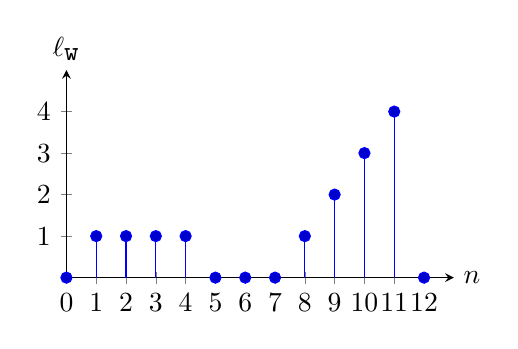
\begin{tikzpicture}
\begin{axis} [width=185pt,height=120pt,
	axis x line=bottom, 
	axis y line=middle, 
	tick align=center,
	every axis x label/.style={at={(current axis.right of origin)},anchor=west},
	every axis y label/.style={at={(current axis.above origin)}, anchor=north east,above=0mm},
	xmin=0, xmax=13,
	xtick={0,...,12},
	xlabel=$n$,
	ymin=0, ymax=5,
	ytick={0,...,4},
	ylabel={$\boldimgworld$}]
\addplot+[ycomb] 
coordinates {(0,0) (1,1) (2,1) (3,1) (4,1) (5,0) (6,0) (7,0) (8,1) (9,2)  (10,3)  (11,4)  (12,0)};
\end{axis}
\end{tikzpicture}
&~
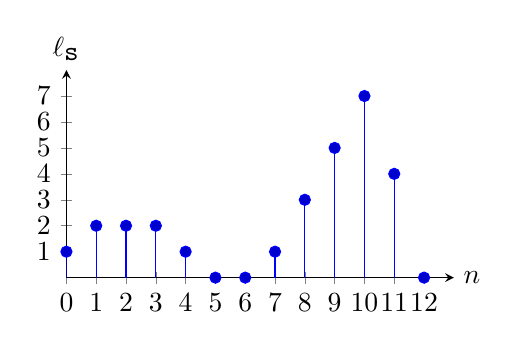
\begin{tikzpicture}
\begin{axis} [width=185pt,height=120pt,
	axis x line=bottom, 
	axis y line=middle, 
	tick align=center,
	every axis x label/.style={at={(current axis.right of origin)},anchor=west},
	every axis y label/.style={at={(current axis.above origin)}, anchor=north east,above=0mm},
	xmin=0, xmax=13,
	xtick={0,...,12},
	xlabel=$n$,
	ymin=0, ymax=8,
	ytick={0,...,7},
	ylabel={$\boldimgsensor$}]
\addplot+[ycomb] 
coordinates {(0,1) (1,2) (2,2) (3,2) (4,1) (5,0) (6,0) (7,1) (8,3) (9,5)  (10,7)  (11,4)  (12,0)};
\end{axis} 
\end{tikzpicture}
\end{array}
$
%\end{center}
}
\caption{Pinhole camera. (left) Input 1D signal, $\boldimgworld$. (right) The output of the two-pixel wide pinhole camera, $\boldimgsensor$.} 
\label{fig:2pixelwidepinhole}
\end{figure}

The output is obtained by multiplying the input vector by the matrix $\mathbf{A}$ shown in \fig{\ref{fig:amats1}}{d}. Each output value is the results of adding up two consecutive input values. The output is nearly identical to the input signal but with a larger magnitude and a bit smoother.

\section{More General Imagers}

Many different optical systems can form cameras and the linear analysis described before can be used to characterize the imaging process.  Even a simple edge will do.  \Fig{\ref{fig:amats3}} shows two non traditional imaging systems that we will analyze in this section. 


\begin{figure}[t]
\centerline{
\includegraphics[width=1\linewidth]{figures/imaging/nontraditional_pinholes_2.eps}
}
\caption{(a) Schematic drawing of an edge camera, and (b) its imaging matrices. (c) A pinspeck camera (an occluder that blocks two of the values on the scene), and (d) its imaging matrices.}
\label{fig:amats3}
\end{figure}

\subsection{Edge Camera}


Consider the example of \fig{\ref{fig:amats3}}{a}. This camera corresponds to an {\bf edge camera}\index{Camera!Edge camera}. This is not a traditional pinhole camera; instead light is blocked only on one side.  




For this camera, the imaging matrix and its inverse are as follows:
%\begin{equation}
%\mathbf{A} = 
%\left( 
%\begin{array}{ccccccccccccc}
%1 & 1 & 1 & 1 & 1 & 1 & 1 & 1 & 1 & 1 & 1 & 1 & 1 \\
%0 & 1 & 1 & 1 & 1 & 1 & 1 & 1 & 1 & 1 & 1 & 1 & 1 \\
%0 & 0 & 1 & 1 & 1 & 1 & 1 & 1 & 1 & 1 & 1 & 1 & 1 \\
%0 & 0 & 0 & 1 & 1 & 1 & 1 & 1 & 1 & 1 & 1 & 1 & 1 \\
%0 & 0 & 0 & 0 & 1 & 1 & 1 & 1 & 1 & 1 & 1 & 1 & 1 \\
%0 & 0 & 0 & 0 & 0 & 1 & 1 & 1 & 1 & 1 & 1 & 1 & 1 \\
%0 & 0 & 0 & 0 & 0 & 0 & 1 & 1 & 1 & 1 & 1 & 1 & 1 \\
%0 & 0 & 0 & 0 & 0 & 0 & 0 & 1 & 1 & 1 & 1 & 1 & 1 \\
%0 & 0 & 0 & 0 & 0 & 0 & 0 & 0 & 1 & 1 & 1 & 1 & 1 \\
%0 & 0 & 0 & 0 & 0 & 0 & 0 & 0 & 0 & 1 & 1 & 1 & 1 \\
%0 & 0 & 0 & 0 & 0 & 0 & 0 & 0 & 0 & 0 & 1 & 1 & 1 \\
%0 & 0 & 0 & 0 & 0 & 0 & 0 & 0 & 0 & 0 & 0 & 1 & 1 \\
%0 & 0 & 0 & 0 & 0 & 0 & 0 & 0 & 0 & 0 & 0 & 0 & 1 
%\end{array}
%\right) .
%\label{eq:edge}
%\end{equation}

\begin{equation}
\mathbf{A} = 
\left[ 
\begin{array}{cccccc}
1 & 1 & 1 & 1 & \dots & 1 \\
0 & 1 & 1 & 1 & ~ & 1 \\
0 & 0 & 1 & 1 & ~ & 1 \\
0 & 0 & 0 & 1 & ~ & 1 \\
\vdots & ~ & ~ & ~ & \ddots & ~ \\
0 & 0 & 0 & 0 & ~ & 1 
\end{array}
\right], 
\mathbf{A}^{-1} = 
\left[ 
\begin{array}{cccccc}
1 & -1 & 0 & 0 & \dots & 0 \\
0 & 1 & -1 & 0 & ~ & 0 \\
0 & 0 & 1 & -1 & ~ & 0 \\
0 & 0 & 0 & 1 & ~ & 0 \\
\vdots & ~ & ~ & ~ & \ddots & ~  \\
0 & 0 & 0 & 0 & ~ & 1 
\end{array}
\right]
\label{eq:edge}
\end{equation}

If we consider the same input as in the pinhole camera example in the previous section, the output signal for the corner camera will look like (\fig{\ref{fig:1dcornercamera}}):

\begin{figure}[h]
\centerline{
%\begin{center}
$
\begin{array}{cc}
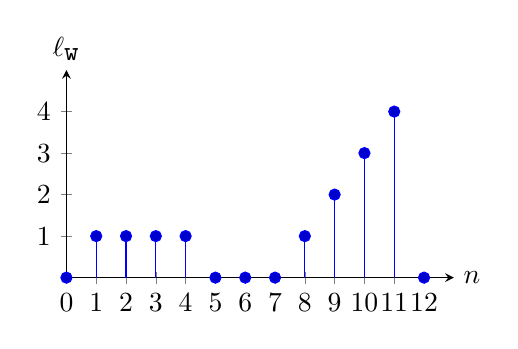
\begin{tikzpicture}
\begin{axis} [width=185pt,height=120pt,
	axis x line=bottom, 
	axis y line=middle, 
	tick align=center,
	every axis x label/.style={at={(current axis.right of origin)},anchor=west},
	every axis y label/.style={at={(current axis.above origin)}, anchor=north east,above=0mm},
	xmin=0, xmax=13,
	xtick={0,...,12},
	xlabel=$n$,
	ymin=0, ymax=5,
	ytick={0,...,4},
	ylabel={$\boldimgworld$}]
\addplot+[ycomb] 
coordinates {(0,0) (1,1) (2,1) (3,1) (4,1) (5,0) (6,0) (7,0) (8,1) (9,2)  (10,3)  (11,4)  (12,0)};
\end{axis}
\end{tikzpicture}
&~
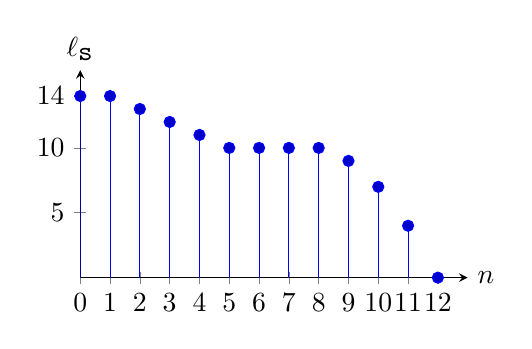
\begin{tikzpicture}
\begin{axis} [width=185pt,height=120pt,
	axis x line=bottom, 
	axis y line=middle, 
	tick align=center,
	every axis x label/.style={at={(current axis.right of origin)},anchor=west},
	every axis y label/.style={at={(current axis.above origin)}, anchor=north east,above=0mm},
	xmin=0, xmax=13,
	xtick={0,...,12},
	xlabel=$n$,
	ymin=0, ymax=16,
	ytick={0,5,10,14},
	ylabel={$\boldimgsensor$}]
\addplot+[ycomb] 
coordinates {(0,14) (1,14) (2,13) (3,12) (4,11) (5,10) (6,10) (7,10) (8,10) (9,9)  (10,7)  (11,4)  (12,0)};
\end{axis} 
\end{tikzpicture}
\end{array}
$
%\end{center}
}
\caption{Edge camera. (left) Input 1D signal, $\boldimgworld$. (right) The output of an edge camera, $\boldimgsensor$.} 
\label{fig:1dcornercamera}
\end{figure}

The output now looks very different than that of a pinhole camera. In the pinhole camera, the output is very similar to the input. This is not the case here where the output looks like the integral of the input (reversed along the horizontal axis). Note that the first value of $\boldimgsensor$ is equal to the sum of all the values of $\boldimgworld$:
\begin{equation}
\imgsensor \left[0 \right] = \sum_{n=0}^{12} \imgworld \left[n \right]
\end{equation}

\Fig{\ref{fig:amats3}}{b} illustrates the imaging matrix, $\mathbf{A}$, and reconstruction matrices for the imager of \eqn{\ref{eq:edge}}. You can think of this imager as computing an integral of the input signal. Therefore, its inverse looks like a derivative. The regularized inverse looks like a blurred derivative (we will talk more about blurred derivatives in \chap{\ref{chapter:image_derivatives}}).
%, as well as for an edge imager where the responses are blurred across several sensor elements.


\subsection{Pinspeck Camera}

\Fig{\ref{fig:amats3}}{c} shows another nontraditional imager. Now, instead of a pinhole we have an occluder. The occluder blocks part of the light (complementary to the large-hole pinhole camera shown in \fig{\ref{fig:amats1}}{c}). What the camera sensor records is the shadow of the occluder.
\marginnote{The shadow of an object is related to the negative of a picture taken of the environment around the object.}
We can write the imaging matrix $\mathbf{A}$, which corresponds to 1-$\mathbf{A}_{pinhole}$ as shown in \fig{\ref{fig:amats1}}{d}. \Fig{\ref{fig:amats3}}{d} also shows its inverse and the regularized inverse. This camera is called a {\bf pinspeck camera}\index{Camera!Pinspeck camera} \cite{CohenPinspeck,Torralba2014} and has also been used in practice. 

In the example of \fig{\ref{fig:amats3}}{c}, the occluder has the size of the wide pinhole from  \fig{\ref{fig:amats1}}{c}. The following plots shows, \fig{\ref{fig:pinspeck_output_plot}}{left}, the input scene (same as in the previous examples) and, \fig{\ref{fig:pinspeck_output_plot}}{right}, the output recorded by the camera sensor of the pinspeck camera. 
\begin{figure}
\centerline{
%\begin{center}
$
\begin{array}{cc}
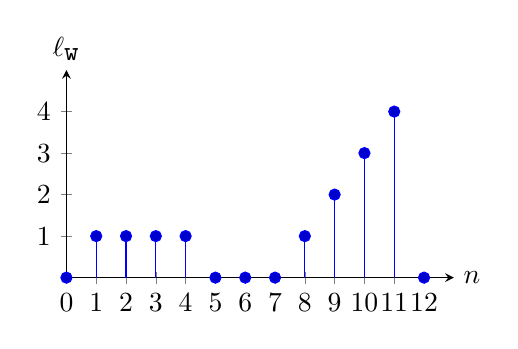
\begin{tikzpicture}
\begin{axis} [width=185pt,height=120pt,
	axis x line=bottom, 
	axis y line=middle, 
	tick align=center,
	every axis x label/.style={at={(current axis.right of origin)},anchor=west},
	every axis y label/.style={at={(current axis.above origin)}, anchor=north east,above=0mm},
	xmin=0, xmax=13,
	xtick={0,...,12},
	xlabel=$n$,
	ymin=0, ymax=5,
	ytick={0,...,4},
	ylabel={$\boldimgworld$}]
\addplot+[ycomb] 
coordinates {(0,0) (1,1) (2,1) (3,1) (4,1) (5,0) (6,0) (7,0) (8,1) (9,2)  (10,3)  (11,4)  (12,0)};
\end{axis}
\end{tikzpicture}
&~
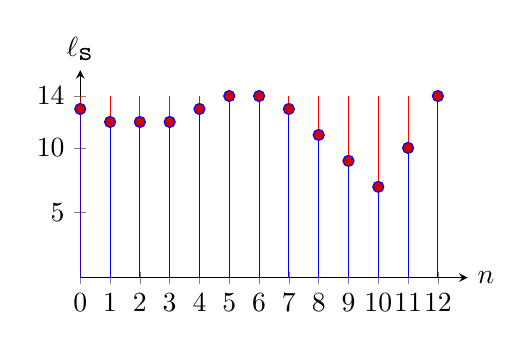
\begin{tikzpicture}
\begin{axis} [width=185pt,height=120pt,
	axis x line=bottom, 
	axis y line=middle, 
	tick align=center,
	every axis x label/.style={at={(current axis.right of origin)},anchor=west},
	every axis y label/.style={at={(current axis.above origin)}, anchor=north east,above=0mm},
	xmin=0, xmax=13,
	xtick={0,...,12},
	xlabel=$n$,
	ymin=0, ymax=16,
	ytick={0,5,10,14},
	ylabel={$\boldimgsensor$}]
\addplot[ycomb,red] 
coordinates {(0,14) (1,14) (2,14) (3,14) (4,14) (5,14) (6,14) (7,14) (8,14) (9,14)  (10,14)  (11,14)  (12,14)};
\addplot+[ycomb,blue,fill=blue,mark=*] 
coordinates {(0,13) (1,12) (2,12) (3,12) (4,13) (5,14) (6,14) (7,13) (8,11) (9,9)  (10,7)  (11,10)  (12,14)};
\end{axis} 
\end{tikzpicture}
\end{array}
$
%\end{center}
}
\caption{Pinspeck camera. (left) Input 1D signal, $\boldimgworld$. (right) The output of a pinspeck camera, $\boldimgsensor$.} 
\label{fig:pinspeck_output_plot}
\end{figure}

The output is now a signal with a wide dynamic range (a max value of 14, which correspond to the sum of the values in $\boldimgworld$) and with fluctuations due to the shadow of the occluder on the camera sensor. If there was no occluder, then the output would be a constant signal of value 14. In red we show the effect of the shadow, which is the light missing because of the presence of the occluder. You can see how the missing signal is identical to the output of the two-pixel wide pinhole camera but reversed in sign.


%\begin{figure}
%\centerline{
%\sublabel{a}{\includegraphics[width=0.45\linewidth]{figures/imaging/ph3.pdf}}}
%\centerline{
%\sublabel{b}{\includegraphics[width=0.45\linewidth]{figures/imaging/amat31.pdf}}
%\sublabel{c}{\includegraphics[width=0.45\linewidth]{figures/imaging/amat34.pdf}}
%}
%\caption{
%(a) An edge camera (b) Visualization of idealized imaging matrices:  The imaging matrix relating scene intensities to sensor readings; the inverse of that matrix;  the regularized inverse.  (c) A blurred edge imaging matrix, and its inverse and regularized inverse }
%\label{fig:amats3}
%\end{figure}





\subsection{Corner Camera}  

To show a real-world example of a more general imager, let us consider the {\bf corner camera}\index{Camera!Corner camera} \cite{Bouman17}.  This is similar to the edge
camera of \eqn{\ref{eq:edge}} and \fig{\ref{fig:amats3}}, but with
slightly more complicated geometry.  As shown in
\fig{\ref{fig:ccmodel}}{a}, a vertical edge partially blocks a scene from view, creating intensity variations on the ground, observable by viewing those intensity variations from around the corner.


\begin{figure}[t]
\centerline{
\sublabel{a}
{\includegraphics[width=0.4\linewidth]{figures/imaging/cornercam.pdf}}
\sublabel{b}
{\includegraphics[width=0.4\linewidth]{figures/imaging/cornerKey.pdf}}}
\caption{The corner camera \cite{Bouman17}.  (a) Objects, such as the cylinders labeled A and B, hidden behind a corner from a camera nonetheless cause a very small intensity differences in the ambient illumination falling on the ground.
%, observable from the camera as a very small change in the light intensity reflecting from the ground.  The image reconstruction operation is analogous to that for the edge camera of \fig{\ref{fig:amats3}}:  we subtract the reflected intensities observed at one orientation angle, say $\theta_A$ from those observed at another, say $\theta_B$. 
(b) the spatial mask is multiplied by the observed reflected ground image.}
\label{fig:ccmodel}
\end{figure}


In practice, we will subtract a mean image from our observations of the ground plane, so in the rendering equation below, we will only consider components of
the scene that may change over time, under the assumption that what we want to image behind the corner (e.g., a person) is moving.  We will call these intensities
$S(\phi, \theta)$ ($S$ for the subject), where $\phi$ measures
vertical inclination and $\theta$ measures azimuthal angle, relative to position where the vertical edge intersects the ground plane.  Integrating the light intensities falling on the ground plane, the
observed intensities on the ground will be $\boldimgground (r, \theta)$, where the
polar coordinates $r$ and $\theta$ are measured with respect to the corner.
Assuming Lambertian diffuse reflection from the ground plane, we have, for the observed intensities $\boldimgground (r, \theta)$,
\begin{equation}
 \boldimgground (r, \theta) = \int_{\phi=0}^{\phi=\pi} \int_{\xi=0}^{\xi=\theta}
 \cos(\phi) S(\phi, \xi) \mbox{d} \phi \mbox{d} \xi,
\label{eq:corner}
\end{equation}
where the $\cos(\phi)$ term in \eqn{\ref{eq:corner}} follows from the equation for surface reflection, \eqn{\ref{eq:lambert}}.



The dependence of the observation, $\boldimgground$, on vertical variations in
$S(\phi, \theta)$ is very weak, just through the $\cos(\phi)$ term.
We can integrate over $\phi$ first, to form the 1D signal,
$\imgworld (\xi)$:
\begin{equation}
  \imgworld (\xi) = \int_{\phi=0}^{\phi=\pi} 
  \cos(\phi) S(\phi, \xi) \mbox{d} \phi 
\label{eq:xcorner}
\end{equation}

Then, to a good approximation, \eqn{\ref{eq:corner}} has the form,
\begin{equation}
 \boldimgground (r, \theta) \approx \int_{\xi=0}^{\xi=\theta}
 \imgworld (\xi) \mbox{d} \xi,
\label{eq:corner1d}
\end{equation}
where $\imgworld (\xi)$ is a 1D image of the scene around the corner from the vertical edge.

\Fig{\ref{fig:ccmodel}} shows the corner camera geometry for a three-dimensional (3D) scene.  \Fig{\ref{fig:ccmodel}}{a} shows two objects, such as the cylinders labeled A and B, hidden behind a corner from a camera. Despite being behind the corner they cause a very small intensity differences in the ambient illumination falling on the ground, observable from the camera as a very small change in the light intensity reflecting from the ground. Can we reconstruct the scene hidden behind the corner using just the intensities observed on the ground? The image reconstruction operation is analogous to that for the edge camera of \fig{\ref{fig:amats3}}:  we subtract the reflected intensities observed at one orientation angle, say $\theta_A$ from those observed at another, say $\theta_B$. 

If we sample \eqn{\ref{eq:corner1d}} in its continuous variables, we
can write it in the form $\boldimgground = \mathbf{A} \boldimgworld$.  Solving \eqn{\ref{eq:deriv2}}
for the multiplier to apply to $\boldimgground$ to estimate $\boldimgworld$ yields the form shown in
\fig{\ref{fig:ccmodel}}{b}.  \Fig{\ref{fig:ccmodel}}{b} shows the spatial mask to be multiplied by the observed reflected ground image, with the result summed over all spatial pixels in order to estimate the light coming from around the corner at one particular orientation angle relative to the corner, in this case approximately 45 degrees. We see that the way to read the 1D signal from the ground plane is to take a derivative with respect to angle.  This makes intuitive sense, as the light intensities on the ground integrate all the light up to the angle of the vertical edge.  To find the 1D signal at the angle of the edge, we ask, ``What does one pie-shaped ray from the wall see that the pie-shaped ray next to it doesn't see?''


It can be shown \cite{Bouman17} that the image intensities from around-the-corner scenes introduce a perturbation of about $\frac{1}{1,000}$ to the light reflected from the ground from all sources.   
By averaging image intensities over the appropriate pie-shaped regions on the ground at the corner (\fig{\ref{fig:ccmodel}}[b]), one can extract a 1D image as a function of time from the scene around the corner.  \Fig{\ref{fig:cctraces}} shows two 1D videos reconstructed from one (\fig{\ref{fig:cctraces}}[a]) and two (\fig{\ref{fig:cctraces}}[b]) people walking around the corner.  By processing videos of very faint intensity changes on the ground, we can infer a 1D video of the scene around the corner.  The image inversion formulas were derived using inversion methods very similar to \eqn{\ref{eq:deriv2}}.  The corner camera is just one of the many possible instantiations of a computational imaging system.


\begin{figure}[t]
\centerline{
\includegraphics[width=0.9\linewidth]{figures/imaging/corner_camera_3D.eps}
}
%\centerline{
%\sublabel{a}
%{\includegraphics[width=0.4\linewidth]{figures/imaging/corner.jpg}}
%\sublabel{b}
%{\includegraphics[width=0.4\linewidth]{figures/imaging/2people.jpg}}}
%\centerline{
%\sublabel{c}
%{\includegraphics[width=0.2\linewidth]{figures/imaging/cctrace.pdf}}
%\sublabel{d}
%{\includegraphics[width=0.2\linewidth]{figures/imaging/cctrace2.pdf}}
%}
\caption{Outdoor corner camera \cite{Bouman17} experiments. (a) Camera recording ground plane intensities.  (b) Two people walking around the corner, hidden from direct view of the camera. (c) Corner camera trace with one person moving. (d) Corner camera trace with two people moving.  Angle from the corner is plotted vertically, and time is plotted horizontally.}
\label{fig:cctraces}
\end{figure}

\marginnote{People moving out of view around a corner cause small, invisible changes in the light reflecting from the ground. These faint changes occur at nearly every corner and can be used to read-out 1D images of the people around the corner.}[0in]


%% 
%% \subsection{Pinhole lightfield imager}
%% An array of pinholes.  How to construct and photograph that?
%% 


\section{Concluding Remarks}  
Treating cameras as general linear systems allows for the machinery of linear algebra to be applied to camera design and processing.  We reviewed several simple camera systems, including cameras utilizing pinholes, pinspecks, and edges to form images.
